\documentclass[10pt,aspectratio=169]{beamer}
\usepackage{../lecture}
\booltrue{wholelecture}

\begin{document}

\begin{frame}
	\titlepage
\end{frame}

\newcommand{\parttocitem}[2]{\item \hyperlink{lecture-#1}{\large\structure{Lecture \lectureroman{#1}: #2}}}

\begin{frame}{Table of Contents}
\begin{itemize}
\parttocitem{1}{Hello, \LaTeX}
%\tableofcontents[part=1,hideallsubsections]
\parttocitem{2}{Text}
\parttocitem{3}{Maths}
\parttocitem{4}{Graphs, Tables and Code}
\end{itemize}
%    \tableofcontents[onlyparts]
\end{frame}

\newlecture{5}{Beamer Slides}

% a tricky fix of nesting frames for documenting beamer itself
% https://tex.stackexchange.com/questions/476964/beamer-verbatim-and-endframe
\newenvironment{fragileframe}{\begin{frame}[fragile,environment=fragileframe]}{\end{frame}}


\section{Introduction}

\subsection{Beamer Document}

\begin{frame}{Why \packagename{beamer}?}

For \LaTeX\ users, \packagename{beamer} has a number of advantages over PowerPoint or other presentation software: \footnote[1]{\url{http://heather.cs.ucdavis.edu/~matloff/beamer.html}}

\begin{itemize}
\item If you are creating slides from a larger document, you can simply re-use your \LaTeX\ source material from that document.
\item If you need mathematical content in your slides, you have the wealth of mathematical constructs in \LaTeX\ to draw upon.
\item The slides you create are multi-platform.
\end{itemize}\medskip

\packagename{beamer} allows you to create slides featuring overlays, animation and so on in \LaTeX. You simply insert some calls to \packagename{beamer} macros in your \LaTeX\ source file, and compile it into a pdf file. You can then use a pdf viewer to present your slides.

\end{frame}

\begin{fragileframe}{The \packagename{beamer} Class}
In order to use \packagename{beamer}, you should use the following command as the first line of your tex document:

\begin{command}
\LC|\documentclass[options]{beamer}|
\end{command}

Then you can create frames with the \packagename{frame} environment or the \LC|\frame| command in the \packagename{document} body.

\begin{example}
\begin{LCL}
\documentclass[options]{beamer}
\begin{document}
\begin{frame}
  some content
\end{frame}
\frame{some content}
\end{document}
\end{LCL}
\end{example}


\end{fragileframe}

\begin{fragileframe}{The Title Page}

You can add title, author, date and some other information in the preamble of the document, similar to the document class \packagename{article}.

\begin{example}
\begin{LCL}
\title{Introduction to \LaTeX}
\author{Liu Yihao}
\date{\today}
\institute{SJTU-UMJI Technology Department}
\end{LCL}
\end{example}

Then you can use the \LC|\titlepage| command to generate a title page.
\begin{command}
\begin{LCL}
\begin{frame}
  \titlepage
\end{frame}
\end{LCL}
\end{command}

This is how the \hyperlink{title-page}{\beamergotobutton{first page}} of this document is generated.

\end{fragileframe}

\begin{fragileframe}

There are some more options for the title page than the ones presented. The next example is a complete one, most of the commands are optional. \footnote[1]{Some of this part is ported from the tutorial of Overleaf: \urllink{https://www.overleaf.com/learn/latex/Beamer}}

\begin{example}
\inputminted[lastline=18]{latex}{../examples/c5/example.tex}
\end{example}

\end{fragileframe}


\begin{fragileframe}

The distribution of each element in the title page depends on the theme, which will be introduced later. Here is a description of each command:

\begin{itemize}
\item \LC|\title[short title]{title}| - The title of your presentation must be inside braces. You can set an optional shorter title in the square brackets.
\item \LC|\subtitle{subtitle}| - Subtitle can be omitted if unnecessary.
\item \LC|\author[short author]{author}| and \LC|\institute[short institute]{institute}| - The usages can be referred to the example code. Use the \LC|\inst| command to state the institute of each author if needed.
\item \LC|\date[short date]{date}| - You can also use \LC|\today| as a date.
\item \LC|\logo{logo}| - You can use text or image, it will be shown on every slide.
\end{itemize} \medskip

The short versions of title, author, institute and date are often used in the headline or footline in the presentation. If omitted, the long versions will be used there. \medskip

The complete example of title page is demonstrated on the next page.

\end{fragileframe}

\begin{fragileframe}
\begin{center}
\LC|\frame{\titlepage}|\medskip

\includegraphics[page=2,width=0.8\textwidth]{../examples/c5/example.pdf}
\end{center}
\end{fragileframe}

\begin{fragileframe}{Frame Title}

You may notice that some of the slides have a title (eg., ``Frame Title'' in this slide). You can use this command to add one:

\begin{command}
\begin{LCL}
\begin{frame}
  \frametitle{frame title}
\end{frame}
\end{LCL}
\end{command}

Alternatively, you can add the title as an argument of the \packagename{frame} environment:

\begin{command}
\begin{LCL}
\begin{frame}{frame title}
  
\end{frame}
\end{LCL}
\end{command}

It is worth noting that in \packagename{beamer} the basic container is a \packagename{frame}. A \packagename{frame} is not exactly equivalent to a slide, one \packagename{frame} may contain more than one slides.

\end{fragileframe}


\subsection{Beamer Structure}

\begin{fragileframe}{Sections and Parts}

You can also structure a \packagename{beamer} document into sections, subsections and subsubsections. Usually subsubsections are not very useful in small presentations.

\begin{command}
\begin{LCL}
\section{section}
\subsection{subsection}
\subsubsection{subsubsection}
\end{LCL}
\end{command}

For large presentations or lectures (such as this one), another structure called \LC|\part| can be used. 

\begin{command}
\begin{LCL}
\part{part}
\end{LCL}
\end{command}

The contents of different parts are often split from each other completely, eg., the counter of figures and tables, the table of contents, etc.

\end{fragileframe}

\begin{fragileframe}{Table of Contents}
After dividing your presentation into sections and subsections, you can add a table of contents at the beginning of the document, or before each section, or anywhere. 

\begin{command}
\begin{LCL}
\begin{frame}{Outline}
  \tableofcontents[options]
\end{frame}
\end{LCL}
\end{command}

For example, if the document structure is
\begin{example}
\begin{multicols}{2}
\begin{LCL}
\section{Section 1}
\subsection{Subsection 1.1}
\subsubsection{Subsubsection 1.1.1}
\subsection{Subsection 1.2}
\subsubsection{Subsubsection 1.2.1}
\subsubsection{Subsubsection 1.2.2}
\section{Section 2}
\subsection{Subsection 2.1}
\subsubsection{Subsubsection 2.1.1}
\subsection{Subsection 2.2}
\subsubsection{Subsubsection 2.2.1}
\subsubsection{Subsubsection 2.2.2}
\end{LCL}
\end{multicols}
\end{example}
An example of the default table of contents is shown on the next page.

\end{fragileframe}

\begin{fragileframe}
\begin{center}
\LC|\frame{\tableofcontents}|\medskip

\includegraphics[page=2,width=0.8\textwidth]{../examples/c5/example.pdf}
\end{center}
\end{fragileframe}


\begin{fragileframe}

By default, all sections, subsections and subsubsections in the current part will be shown in the table and contents. You can also use options to set whether some of the sections or subsections should be shaded, or be hided. The allowed styles are \structure{show}, \structure{shaded} and \structure{hide}. The available options are 

\begin{itemize}
\item \structure{\LC|sectionstyle=<style for current section>/<style for other sections>|}
\item \structure{\LC|subsectionstyle=<style for current subsection>/<style for other subsections in current section>/<style for subsections in other sections>|}
\item \structure{\LC|subsubsectionstyle=<style for current subsubsection>/<style for other subsubsections in current
subsection>/<style for subsubsections in other subsections in current section>/<style for subsubsections in other
subsections in other sections>|}\medskip
\end{itemize}

The later styles can be omitted in each options, in this case, the omitted styles will be set to the last explicit style. For example, these two lines are equivalent:

\begin{itemize}
\item \structure{\LC|subsectionstyle=show/shaded|}
\item \structure{\LC|subsectionstyle=show/shaded/shaded|}
\end{itemize}

They both cause all subsections except the current subsection in the
current section to be shown in a semi-transparent way.

\end{fragileframe}

\begin{fragileframe}

There are also some shorthands of the options above, you can use them alone, or mix them with any other options.

\begin{itemize}
\item \structure{\LC|currentsection|} - \LC|sectionstyle=show/shaded,subsectionstyle=show/show/shaded|
\item \structure{\LC|currentsubsection|} - \LC|subsectionstyle=show/shaded|
\item \structure{\LC|hideallsubsections|} - \LC|subsectionstyle=hide|
\item \structure{\LC|hideothersubsections|} - \LC|subsectionstyle=show/show/hide|
\end{itemize}\medskip

Some other options include
\begin{itemize}
\item \structure{\LC|part=<part number>|} - shows the table of contents of a specific part.
\item \structure{\LC|pausesections|} - causes a \LC|\pause| command to be issued before each section. This is useful if you wish
to show the table of contents in an incremental way.
\item \structure{\LC|pausesubsections|} - causes a \LC|\pause| command to be issued before each subsection.
\end{itemize}\medskip

The \LC|\pause| command can split a frame into two slides, which will be introduced in the next section. \medskip

Some examples are shown on the next pages.

\end{fragileframe}

\begin{fragileframe}
\begin{center}
\LC|\frame{\tableofcontents[pausesection]}|\medskip

\includegraphics<1>[page=3,width=0.75\textwidth]{../examples/c5/example.pdf}
\includegraphics<2>[page=4,width=0.75\textwidth]{../examples/c5/example.pdf}
\end{center}
\end{fragileframe}

\begin{fragileframe}
\begin{center}
\LC|\frame{\tableofcontents[currentsection]}|\medskip

\includegraphics[page=5,width=0.75\textwidth]{../examples/c5/example.pdf}
\end{center}
\end{fragileframe}

\begin{fragileframe}
\begin{center}
\LC|\frame{\tableofcontents[currentsubsection]}|\medskip

\includegraphics[page=6,width=0.75\textwidth]{../examples/c5/example.pdf}
\end{center}
\end{fragileframe}

\begin{fragileframe}
\begin{center}
\LC|\frame{\tableofcontents[sectionstyle=show/shaded,
subsectionstyle=show/shaded/hide,subsubsectionstyle=show/shaded/hide]}|\medskip

\includegraphics[page=7,width=0.75\textwidth]{../examples/c5/example.pdf}
\end{center}
\end{fragileframe}

\begin{fragileframe}{Bibliography}

Like the \packagename{article} class, you can use \LC|\cite| to create citations and add a bibliography at the end of the file. \medskip

Unfortunately, \packagename{bibtex} is not perfectly supported in \packagename{beamer}, so usually you need to typeset them by hand.

\begin{example}
\begin{LCL}
\begin{frame}
  \frametitle{For Further Reading}
  \begin{thebibliography}{Dijkstra, 1982}
    \bibitem[Salomaa, 1973]{Salomaa1973} A.~Salomaa.
    \newblock {\em Formal Languages}. \newblock Academic Press, 1973.
    \bibitem[Dijkstra, 1982]{Dijkstra1982} E.~Dijkstra. 
    \newblock Smoothsort, an alternative for sorting in situ. 
    \newblock {\em Science of Computer Programming}, 1(3):223--233, 1982. 
  \end{thebibliography} 
\end{frame}
\end{LCL}
\end{example}


\end{fragileframe}

\begin{fragileframe}{Appendix}

You can add an appendix by using the \LC|\appendix| command. The  command essentially just starts a new part named \LC|\appendixname|. However, it also sets up certain hyperlinks. \medskip

All frames, all \LC|\subsection| commands, and all \LC|\section| commands used after this command will not be shown as part of the normal navigation bars. 

\begin{example}
\begin{multicols}{2}
\begin{LCL}
\begin{document}
\frame{\titlepage}
\section*{Outline} 
\frame{\tableofcontents} 
\section{Main Text} 
\frame{Some text} 
\section*{Summary} 
\frame{Summary text}

 
\appendix 
\section{\appendixname} 
\frame{\tableofcontents} 
\subsection{Additional material} 
\frame{Details} 
\frame{Text omitted in main talk.} 
\subsection{Even more additional material} 
\frame{More details} 
\end{document}
\end{LCL}
\end{multicols}
\end{example}

\end{fragileframe}


\section{Overlay and Animation}

\subsection{Overlay}

\begin{fragileframe}{Simple Overlay}

In the introduction, it was mentioned that a frame is not equivalent to a slide. \medskip

\pause

The simplest way to verify this is to add a simple overlay with the command

\begin{command}
\begin{LCL}
\pause
\end{LCL}
\end{command}

\pause

A direct example is this frame itself:
\begin{example}
\begin{LCL}
\begin{frame}{Simple Overlay}
  some contents
  \pause
  some contents
  \pause
  some contents
\end{frame}
\end{LCL}
\end{example}

Note that the page numbers in the bottom right corner of these three slides are the same, the page counter only counts the number of frames.

\end{fragileframe}

\begin{fragileframe}{Overlay Specifications}

However, the \LC|\pause| command only provide a basic support of splitting slides. Using commands with an overlay specification will be more flexible, which means you can have different effects with the same command on different slides. \medskip

Overlay specifications can only be written behind certain commands, not every command. \LC|\textbf| is one of these commands.

\begin{latexexample}
\textbf{This line is bold on all slides.}
\textbf<2>{This line is bold only on the second slide.}
\end{latexexample}

The syntax of (basic) overlay specifications is the following: They are comma-separated lists of slides and
ranges. Ranges are specified like this: \packagename{2-5}, which means slide two through to five. \medskip

The start or the end of a range can be omitted. For example, \packagename{3-} means ``slides three, four, five, and so on''.

\end{fragileframe}


\begin{fragileframe}

For the following commands, adding an overlay specification causes the command to be simply ignored on slides that are not included in the specification: \LC|\textbf|, \LC|\textit|, \LC|\textmd|, \LC|\textnormal|, \LC|\textrm|, \LC|\textsc|,
\LC|\textsf|, \LC|\textsl|, \LC|\texttt|, \LC|\textup|, \LC|\emph|, \LC|\color|, \LC|\textcolor|, \LC|\alert|, \LC|\structure|. If a command takes
several arguments, like \LC|\color|, the specification should directly follow the command.

\begin{latexexample}
\color<2>[rgb]{1,0,0} This text is red on slides 2, otherwise black.
\end{latexexample}

\end{fragileframe}


\begin{fragileframe}{The \packagename{onslide} Command}

When you want to display or hide some contents on some slides, you can use

\begin{command}
\LC|\onslide(modifier)<overlay specification>{text}|
\end{command}

\begin{latexexample}
\onslide<1>{(1) onslide}
\uncover<1>{(1) uncover}

\onslide+<2>{(2) onslide+}
\visible<2>{(2) visible}

\onslide*<3>{(3) onslide*}
\only<3>{(3) only}
\end{latexexample}

\end{fragileframe}

\begin{fragileframe}

Some explanations:

\begin{itemize}
\item \LC|\onslide| is equivalent to \LC|\uncover|, the text is only shown (``uncovered'') on the specified slides. On other slides, \alert{the text still occupies space} and it is still typeset, but it is not shown or only shown as if transparent (can be set with the command \LC|\setbeamercovered|).
\item \LC|\onslide+| is equivalent to \LC|\visible|, it does almost the same as \LC|\uncover|, but it is never transparent, but rather it is not shown at all.
\item \LC|\onslide*| is equivalent to \LC|\only|, the text is inserted only into
the specified slides. For other slides, the text is simply thrown away. In particular, \alert{it occupies no space}.
\end{itemize}

There are also some similar commands:

\begin{itemize}
\item \LC|\invisible<overlay specification>{text}| is opposite to \LC|\visible|.
\item \LC|\alt<overlay specification>{text}{alternate text}| will show the text on the specified slides and the alternate text on other slides.
\item \LC|\temporal<overlay specification>{before text}{text}{after text}| will show the text on the specified slides, the before text on the slides before the interval, and the after text on the slides after the interval.
\end{itemize}

\end{fragileframe}

\subsection{Animation}


\begin{fragileframe}{Zooming}

Zooming is necessary when you want to explain a part of a frame (or a very complicated graphic).

\begin{command}
\LC|\framezoom<button overlay specification><zoomed overlay specification>[options](x,y)(w,d)|
\end{command}

This command should be given somewhere at the beginning of a frame. The button overlay specification is your main slide with the whole graph, and there will be a clickable area which will navigate you to the zoomed slide, specified by the zoomed overlay. \medskip

\packagename{(x,y)} is the upper left corner of the clickable area. Thus,
the location \packagename{(0pt,0pt)} is at the beginning of the normal text (which excludes the headline and also the frame title). \packagename{(w,d)} is the width and depth (height) of the clickable area. \medskip

You can also add \LC|border=width| as \packagename{options} so that there will be a border around the clickable area.

\end{fragileframe}

\begin{fragileframe}

\begin{latexexample}
\framezoom<1><2>(0cm,0cm)(4cm,3cm)
\framezoom<1><3>(1.5cm,3.5cm)(4cm,3cm)
\pgfimage[height=5cm]{example-image}
\end{latexexample}

Try to click on the code and the image.

\end{fragileframe}

\begin{fragileframe}{Limitations of Zooming}

Though \LC|\framezoom| is very powerful, it still has some limitations.

\begin{itemize}
\item You can click on the zoomed slide to jump back to the origin slide, but it only works on Adobe Reader or Acrobat.
\item The backend of \XeLaTeX\ will ignore all hyperlinks without text in it, so when compiling with \packagename{xelatex}, the area is no longer clickable. You can use \packagename{pdflatex} or \packagename{lualatex} when you need the zooming feature. \medskip

You can also redefine some macros in the \packagename{beamer} package to use \packagename{xelatex} with expected behavior, but it will require some knowledge of the inner concept of \LaTeX. You can check \href{https://github.com/SJTU-UMJI-Tech/LaTeX/blob/master/lecture/lecture.sty}{\packagename{lecture.sty}} for more details.
\end{itemize}

\end{fragileframe}

\begin{fragileframe}{The \packagename{againframe} Command}
	
You can use the \LC|\againframe| command to ``continue'' frames that you previously started
somewhere, but where certain details have been suppressed. You need to add a label for the frame to be repeated.

\begin{command}
\LC|\againframe<overlay specification>[options]{label}|
\end{command}

You can use this command together with the \LC|\framezoom| command to put the zoomed slides at the end of the presentation.

\begin{example}
\begin{LCL}
\begin{frame}<1>[label=zooms]
\frametitle<1>{A Complicated Picture}
\framezoom<1><2>[border](0cm,0cm)(2cm,1.5cm)
\framezoom<1><3>[border](1cm,2cm)(2cm,1.5cm)
\pgfimage[height=6cm]{example-image}
\end{frame}
% other slides
\againframe<2->[noframenumbering]{zooms}
\end{LCL}
\end{example}

\end{fragileframe}


\begin{frame}<1>[label=zooms]
\frametitle<1>{A Complicated Picture}
\framezoom<1><2>[border](0cm,0cm)(2cm,1.5cm)
\framezoom<1><3>[border](1cm,2cm)(2cm,1.5cm)
\pgfimage[height=6cm]{example-image}
\end{frame}

\section{Special Structures}

\subsection{Blocks and Columns}

\begin{fragileframe}{The \packagename{block} Environment}

Blocks in \packagename{beamer} are based on the \packagename{tcolorbox}, with all styles configured.

\begin{command}
\begin{LCL}
\begin{block}<action specification>{title}
  % block contents
\end{block}
\end{LCL}
\end{command}

If the \packagename{action specification} is present, the given actions are taken on the specified slides. \medskip

There are three types of blocks: \packagename{block}, \packagename{alertblock} and \packagename{exampleblock}. The only difference is their color and style.

\end{fragileframe}


\begin{fragileframe}

\begin{example}
\begin{LCL}
\begin{block}{Normal Block}
  This is a normal block.
\end{block}
\begin{alertblock}{Alert Block}
  This is an alert block.
\end{alertblock}
\begin{exampleblock}{Example Block}
  This is an example block.
\end{exampleblock}
\end{LCL}
\end{example}

\begin{block}{Normal Block}
  This is a normal block.
\end{block}

\begin{alertblock}{Alert Block}
  This is an alert block.
\end{alertblock}

\begin{exampleblock}{Example Block}
  This is an example block.
\end{exampleblock}

\end{fragileframe}


\begin{fragileframe}{Predefined block environments}

Some other block environment are predefined for ease to use. They are \packagename{theorem}, \packagename{corollary}, \packagename{definition}, \packagename{definitions}, \packagename{example}, \packagename{examples}. Here only a few of them are shown below.


\begin{example}
\begin{LCL}
\begin{theorem}[additional text]
  The additional text will be in brackets if the option is provided.
\end{theorem}
\begin{proof}[Proof Name]
  The default title is ``Proof.'', which can be replaced by the option.
\end{proof}
\end{LCL}
\end{example}

\begin{theorem}[additional text]
  The additional text will be in brackets if the option is provided.
\end{theorem}
\begin{proof}[Proof Name]
  The default title is ``Proof.'', which can be replaced by the option.
\end{proof}

\end{fragileframe}

\begin{fragileframe}{The \packagename{columns} Environment}

In an \packagename{article} class, \packagename{minipage} is often used to split contents into multiple columns; In \packagename{beamer}, you can use the \packagename{columns} environment as an alternative. 

\begin{command}
\begin{LCL}
\begin{columns}[options]
  \begin{column}[placement]{width}
    % contents
  \end{column}
  \column[placement]{width}{...}
\end{columns} 
\end{LCL}
\end{command}

For the \packagename{options} in the \packagename{columns} environment,

\begin{itemize}
\item \structure{\LC|b|}, \structure{\LC|c|} and \structure{\LC|t|} -  will cause the columns to be vertically aligned \packagename{bottom}, \packagename{center} and \packagename{top}.
\item \structure{\LC|T|} - similar to \structure{\LC|t|}, if strange things happen in \structure{\LC|t|}, try this option.
\item \structure{\LC|totalwidth=width|} -  will cause the columns to occupy not the whole page width, but only \packagename{width}.
\end{itemize}\medskip

\end{fragileframe}

\begin{fragileframe}

\begin{latexexample}
\begin{columns}[c]
  \begin{column}{0.5\textwidth}
    \begin{center}
      The first line \\
      The second line
    \end{center}
  \end{column}
  \column{0.5\textwidth}{
    \includegraphics[width=0.6\textwidth]{example-image}
  }
\end{columns} 
\end{latexexample}

\end{fragileframe}

\begin{fragileframe}

You should place only \packagename{column} environments or \LC|\column| commands in the \packagename{columns} environment. \medskip

For the \packagename{placement} in the \packagename{column} environment or the \LC|\column| command, you can overwrite the \structure{\LC|b|}, \structure{\LC|c|}, \structure{\LC|t|} and \structure{\LC|T|} in the outer \packagename{columns} environment. The default of \packagename{placement} is \structure{\LC|t|} if not specified. \medskip

The \packagename{width} is the same as other \packagename{width} in \LaTeX. For example, you can use \LC|5cm|, or \LC|\textwidth|. \bigskip

Generally speaking, there are few differences between \packagename{minipage} and \packagename{columns}, but the \packagename{columns} environment has a more user-friendly structure, and overlap is supported better in it. Despite which do you prefer, choosing one of them and sticking to it throughout a presentation is suggested.

\end{fragileframe}

\begin{fragileframe}{Footnote in \packagename{column}}

Using footnotes is usually not a good idea. They disrupt the flow of reading. \medskip

When you really need it, you can use the \LC|\footnote| command, which is slightly different from common \LaTeX. \medskip

\begin{command}
\LC|\footnote<overlay specification>[options]{text}|
\end{command}

As usual, you can give a number as \packagename{options}, which will cause the footnote to use that number. \medskip

You can also add a \packagename{frame} as \packagename{options} so that the footnote will be shown at the bottom of the frame. This is normally the default behavior anyway, but in \packagename{minipage}, \packagename{columns} and certain blocks it makes a difference. \medskip

In a \packagename{minipage} or \packagename{column}, the footnote is usually shown as part of the minipage rather than as part of the frame. 

\end{fragileframe}

\begin{fragileframe}

\begin{latexexample}
\begin{columns}[c,totalwidth=0.9\textwidth]
  \begin{column}{0.3\textwidth}
    The first line \footnote[frame,1]{footnote 1}
  \end{column}
  \begin{column}{0.3\textwidth}
    The second line \footnote[frame,2]{footnote 2}
  \end{column}
  \begin{column}{0.3\textwidth}
    The third line \footnote[3]{footnote 3}
  \end{column}
\end{columns} 
\end{latexexample}

As you can see, placing footnote at the bottom of a \packagename{column} is not a good idea, so using the \packagename{frame} option is preferred in most situations.

\end{fragileframe}

\subsection{Hyperlinks and Buttons}

\begin{fragileframe}{Hyperlinks and Buttons}

Here is a simple three-step workflow of how to create hyperlinks and buttons in your slides: \medskip

\begin{enumerate}

\item You specify a target using the command \LC|\hypertarget| or (easier) the command \LC|\label|. In some cases, see below, this step may be skipped. 

\item You render the button using \LC|\beamerbutton| or a similar command. This will render the button, but clicking it will not yet have any effect. 

\item You put the button inside a \LC|\hyperlink| command. Now clicking it will jump to the target of the link. 

\end{enumerate}

\end{fragileframe}


\begin{fragileframe}{The \packagename{beamerbutton} command}

\begin{command}
\LC|\beamerbutton{text}|
\end{command}

There are four types of buttons, the suggested usages of them are:

\begin{itemize}
\item \LC|\beamerbutton| - a normal button
\item \LC|\beamergotobutton| - jump to another area of the presentation
\item \LC|\beamerskipbutton| - skip a well-defined part
\item \LC|\beamerreturnbutton| - return back to a previous part
\end{itemize}

\begin{latexexample}
\beamerbutton{normal}   \beamergotobutton{goto}
\beamerskipbutton{skip} \beamerreturnbutton{return}
\end{latexexample}

The color of the buttons will follow the current color of the block.

\beamerbutton{normal}
\beamergotobutton{goto}
\beamerskipbutton{skip}
\beamerreturnbutton{return}



\end{fragileframe}


\begin{fragileframe}{The \packagename{hyperlink} command}
\begin{command}
\LC|\hyperlink<overlay specification>{target}{text}|
\end{command}

If the overlay specification is present, the hyperlink (including the text) is completely suppressed on the non-specified slides. \medskip

You will jump to the \packagename{target} you defined before with a \LC|\hypertarget| command. \bigskip

You can also use a \LaTeX\ command from the \packagename{hyperref} package as a target, e.g., \LC|\href|.

\begin{latexexample}
You can find the source of the slides on 
\href{https://github.com/SJTU-UMJI-Tech/LaTeX}{\beamerbutton{GitHub}}.
\end{latexexample}

\end{fragileframe}


\begin{fragileframe}{The \packagename{hypertarget} command}

\begin{command}
\LC|\hypertarget<overlay specification>{target}{text}|
\end{command}

If the overlay specification is present, the text is the target for hyper jumps only on the specified slide. On all other slides, the text is shown normally.

\begin{latexexample}
\begin{itemize}
  \item<1-> First item.
  \item<2-> Second item.
\end{itemize}
\hyperlink{jumptosecond}{\beamergotobutton{Jump to second slide}}
\hypertarget<2>{jumptosecond}{}
\end{latexexample}

\end{fragileframe}



\subsection{Fragile Frame}

\begin{fragileframe}{Fragile Frame}

When you need to insert any verbatim (such as \packagename{minted}) in a frame, you have to add the option \LC|[fragile]|, and the \LC|\end{frame}| must be alone on a single line (except for any leading whitespace).

\begin{example}
\begin{LCL}
\begin{frame}[fragile]
  \begin{minted}{latex}
\documentclass{beamer}
  \end{minted}
\end{frame}
\end{LCL}
\end{example}

Using this option will cause the frame contents to be written to an external file and then read back. 

\end{fragileframe}

\begin{fragileframe}{Frame in Fragile Frame}

A more tricky situation is that you want to put \LC|\begin{frame}| and \LC|\end{frame}| inside a verbatim environment (like this lecture). \medskip

One possible solution is to define a new environment so that the new environment name won't conflict with the content in the verbatim environment.

\begin{example}
\begin{LCL}
\newenvironment{fragileframe}%
{\begin{frame}[fragile,environment=fragileframe]}%
{\end{frame}}
\end{LCL}
\end{example}

Then you can use \LC{\begin{fragileframe}} to substitute \LC{\begin{frame}[fragile]} for all fragile frames.

\end{fragileframe}

\againframe<2->[noframenumbering]{zooms}





\newlecture{5}{Beamer Slides}

% a tricky fix of nesting frames for documenting beamer itself
% https://tex.stackexchange.com/questions/476964/beamer-verbatim-and-endframe
\newenvironment{fragileframe}{\begin{frame}[fragile,environment=fragileframe]}{\end{frame}}


\section{Introduction}

\subsection{Beamer Document}

\begin{frame}{Why \packagename{beamer}?}

For \LaTeX\ users, \packagename{beamer} has a number of advantages over PowerPoint or other presentation software: \footnote[1]{\url{http://heather.cs.ucdavis.edu/~matloff/beamer.html}}

\begin{itemize}
\item If you are creating slides from a larger document, you can simply re-use your \LaTeX\ source material from that document.
\item If you need mathematical content in your slides, you have the wealth of mathematical constructs in \LaTeX\ to draw upon.
\item The slides you create are multi-platform.
\end{itemize}\medskip

\packagename{beamer} allows you to create slides featuring overlays, animation and so on in \LaTeX. You simply insert some calls to \packagename{beamer} macros in your \LaTeX\ source file, and compile it into a pdf file. You can then use a pdf viewer to present your slides.

\end{frame}

\begin{fragileframe}{The \packagename{beamer} Class}
In order to use \packagename{beamer}, you should use the following command as the first line of your tex document:

\begin{command}
\LC|\documentclass[options]{beamer}|
\end{command}

Then you can create frames with the \packagename{frame} environment or the \LC|\frame| command in the \packagename{document} body.

\begin{example}
\begin{LCL}
\documentclass[options]{beamer}
\begin{document}
\begin{frame}
  some content
\end{frame}
\frame{some content}
\end{document}
\end{LCL}
\end{example}


\end{fragileframe}

\begin{fragileframe}{The Title Page}

You can add title, author, date and some other information in the preamble of the document, similar to the document class \packagename{article}.

\begin{example}
\begin{LCL}
\title{Introduction to \LaTeX}
\author{Liu Yihao}
\date{\today}
\institute{SJTU-UMJI Technology Department}
\end{LCL}
\end{example}

Then you can use the \LC|\titlepage| command to generate a title page.
\begin{command}
\begin{LCL}
\begin{frame}
  \titlepage
\end{frame}
\end{LCL}
\end{command}

This is how the \hyperlink{title-page}{\beamergotobutton{first page}} of this document is generated.

\end{fragileframe}

\begin{fragileframe}

There are some more options for the title page than the ones presented. The next example is a complete one, most of the commands are optional. \footnote[1]{Some of this part is ported from the tutorial of Overleaf: \urllink{https://www.overleaf.com/learn/latex/Beamer}}

\begin{example}
\inputminted[lastline=18]{latex}{../examples/c5/example.tex}
\end{example}

\end{fragileframe}


\begin{fragileframe}

The distribution of each element in the title page depends on the theme, which will be introduced later. Here is a description of each command:

\begin{itemize}
\item \LC|\title[short title]{title}| - The title of your presentation must be inside braces. You can set an optional shorter title in the square brackets.
\item \LC|\subtitle{subtitle}| - Subtitle can be omitted if unnecessary.
\item \LC|\author[short author]{author}| and \LC|\institute[short institute]{institute}| - The usages can be referred to the example code. Use the \LC|\inst| command to state the institute of each author if needed.
\item \LC|\date[short date]{date}| - You can also use \LC|\today| as a date.
\item \LC|\logo{logo}| - You can use text or image, it will be shown on every slide.
\end{itemize} \medskip

The short versions of title, author, institute and date are often used in the headline or footline in the presentation. If omitted, the long versions will be used there. \medskip

The complete example of title page is demonstrated on the next page.

\end{fragileframe}

\begin{fragileframe}
\begin{center}
\LC|\frame{\titlepage}|\medskip

\includegraphics[page=2,width=0.8\textwidth]{../examples/c5/example.pdf}
\end{center}
\end{fragileframe}

\begin{fragileframe}{Frame Title}

You may notice that some of the slides have a title (eg., ``Frame Title'' in this slide). You can use this command to add one:

\begin{command}
\begin{LCL}
\begin{frame}
  \frametitle{frame title}
\end{frame}
\end{LCL}
\end{command}

Alternatively, you can add the title as an argument of the \packagename{frame} environment:

\begin{command}
\begin{LCL}
\begin{frame}{frame title}
  
\end{frame}
\end{LCL}
\end{command}

It is worth noting that in \packagename{beamer} the basic container is a \packagename{frame}. A \packagename{frame} is not exactly equivalent to a slide, one \packagename{frame} may contain more than one slides.

\end{fragileframe}


\subsection{Beamer Structure}

\begin{fragileframe}{Sections and Parts}

You can also structure a \packagename{beamer} document into sections, subsections and subsubsections. Usually subsubsections are not very useful in small presentations.

\begin{command}
\begin{LCL}
\section{section}
\subsection{subsection}
\subsubsection{subsubsection}
\end{LCL}
\end{command}

For large presentations or lectures (such as this one), another structure called \LC|\part| can be used. 

\begin{command}
\begin{LCL}
\part{part}
\end{LCL}
\end{command}

The contents of different parts are often split from each other completely, eg., the counter of figures and tables, the table of contents, etc.

\end{fragileframe}

\begin{fragileframe}{Table of Contents}
After dividing your presentation into sections and subsections, you can add a table of contents at the beginning of the document, or before each section, or anywhere. 

\begin{command}
\begin{LCL}
\begin{frame}{Outline}
  \tableofcontents[options]
\end{frame}
\end{LCL}
\end{command}

For example, if the document structure is
\begin{example}
\begin{multicols}{2}
\begin{LCL}
\section{Section 1}
\subsection{Subsection 1.1}
\subsubsection{Subsubsection 1.1.1}
\subsection{Subsection 1.2}
\subsubsection{Subsubsection 1.2.1}
\subsubsection{Subsubsection 1.2.2}
\section{Section 2}
\subsection{Subsection 2.1}
\subsubsection{Subsubsection 2.1.1}
\subsection{Subsection 2.2}
\subsubsection{Subsubsection 2.2.1}
\subsubsection{Subsubsection 2.2.2}
\end{LCL}
\end{multicols}
\end{example}
An example of the default table of contents is shown on the next page.

\end{fragileframe}

\begin{fragileframe}
\begin{center}
\LC|\frame{\tableofcontents}|\medskip

\includegraphics[page=2,width=0.8\textwidth]{../examples/c5/example.pdf}
\end{center}
\end{fragileframe}


\begin{fragileframe}

By default, all sections, subsections and subsubsections in the current part will be shown in the table and contents. You can also use options to set whether some of the sections or subsections should be shaded, or be hided. The allowed styles are \structure{show}, \structure{shaded} and \structure{hide}. The available options are 

\begin{itemize}
\item \structure{\LC|sectionstyle=<style for current section>/<style for other sections>|}
\item \structure{\LC|subsectionstyle=<style for current subsection>/<style for other subsections in current section>/<style for subsections in other sections>|}
\item \structure{\LC|subsubsectionstyle=<style for current subsubsection>/<style for other subsubsections in current
subsection>/<style for subsubsections in other subsections in current section>/<style for subsubsections in other
subsections in other sections>|}\medskip
\end{itemize}

The later styles can be omitted in each options, in this case, the omitted styles will be set to the last explicit style. For example, these two lines are equivalent:

\begin{itemize}
\item \structure{\LC|subsectionstyle=show/shaded|}
\item \structure{\LC|subsectionstyle=show/shaded/shaded|}
\end{itemize}

They both cause all subsections except the current subsection in the
current section to be shown in a semi-transparent way.

\end{fragileframe}

\begin{fragileframe}

There are also some shorthands of the options above, you can use them alone, or mix them with any other options.

\begin{itemize}
\item \structure{\LC|currentsection|} - \LC|sectionstyle=show/shaded,subsectionstyle=show/show/shaded|
\item \structure{\LC|currentsubsection|} - \LC|subsectionstyle=show/shaded|
\item \structure{\LC|hideallsubsections|} - \LC|subsectionstyle=hide|
\item \structure{\LC|hideothersubsections|} - \LC|subsectionstyle=show/show/hide|
\end{itemize}\medskip

Some other options include
\begin{itemize}
\item \structure{\LC|part=<part number>|} - shows the table of contents of a specific part.
\item \structure{\LC|pausesections|} - causes a \LC|\pause| command to be issued before each section. This is useful if you wish
to show the table of contents in an incremental way.
\item \structure{\LC|pausesubsections|} - causes a \LC|\pause| command to be issued before each subsection.
\end{itemize}\medskip

The \LC|\pause| command can split a frame into two slides, which will be introduced in the next section. \medskip

Some examples are shown on the next pages.

\end{fragileframe}

\begin{fragileframe}
\begin{center}
\LC|\frame{\tableofcontents[pausesection]}|\medskip

\includegraphics<1>[page=3,width=0.75\textwidth]{../examples/c5/example.pdf}
\includegraphics<2>[page=4,width=0.75\textwidth]{../examples/c5/example.pdf}
\end{center}
\end{fragileframe}

\begin{fragileframe}
\begin{center}
\LC|\frame{\tableofcontents[currentsection]}|\medskip

\includegraphics[page=5,width=0.75\textwidth]{../examples/c5/example.pdf}
\end{center}
\end{fragileframe}

\begin{fragileframe}
\begin{center}
\LC|\frame{\tableofcontents[currentsubsection]}|\medskip

\includegraphics[page=6,width=0.75\textwidth]{../examples/c5/example.pdf}
\end{center}
\end{fragileframe}

\begin{fragileframe}
\begin{center}
\LC|\frame{\tableofcontents[sectionstyle=show/shaded,
subsectionstyle=show/shaded/hide,subsubsectionstyle=show/shaded/hide]}|\medskip

\includegraphics[page=7,width=0.75\textwidth]{../examples/c5/example.pdf}
\end{center}
\end{fragileframe}

\begin{fragileframe}{Bibliography}

Like the \packagename{article} class, you can use \LC|\cite| to create citations and add a bibliography at the end of the file. \medskip

Unfortunately, \packagename{bibtex} is not perfectly supported in \packagename{beamer}, so usually you need to typeset them by hand.

\begin{example}
\begin{LCL}
\begin{frame}
  \frametitle{For Further Reading}
  \begin{thebibliography}{Dijkstra, 1982}
    \bibitem[Salomaa, 1973]{Salomaa1973} A.~Salomaa.
    \newblock {\em Formal Languages}. \newblock Academic Press, 1973.
    \bibitem[Dijkstra, 1982]{Dijkstra1982} E.~Dijkstra. 
    \newblock Smoothsort, an alternative for sorting in situ. 
    \newblock {\em Science of Computer Programming}, 1(3):223--233, 1982. 
  \end{thebibliography} 
\end{frame}
\end{LCL}
\end{example}


\end{fragileframe}

\begin{fragileframe}{Appendix}

You can add an appendix by using the \LC|\appendix| command. The  command essentially just starts a new part named \LC|\appendixname|. However, it also sets up certain hyperlinks. \medskip

All frames, all \LC|\subsection| commands, and all \LC|\section| commands used after this command will not be shown as part of the normal navigation bars. 

\begin{example}
\begin{multicols}{2}
\begin{LCL}
\begin{document}
\frame{\titlepage}
\section*{Outline} 
\frame{\tableofcontents} 
\section{Main Text} 
\frame{Some text} 
\section*{Summary} 
\frame{Summary text}

 
\appendix 
\section{\appendixname} 
\frame{\tableofcontents} 
\subsection{Additional material} 
\frame{Details} 
\frame{Text omitted in main talk.} 
\subsection{Even more additional material} 
\frame{More details} 
\end{document}
\end{LCL}
\end{multicols}
\end{example}

\end{fragileframe}


\section{Overlay and Animation}

\subsection{Overlay}

\begin{fragileframe}{Simple Overlay}

In the introduction, it was mentioned that a frame is not equivalent to a slide. \medskip

\pause

The simplest way to verify this is to add a simple overlay with the command

\begin{command}
\begin{LCL}
\pause
\end{LCL}
\end{command}

\pause

A direct example is this frame itself:
\begin{example}
\begin{LCL}
\begin{frame}{Simple Overlay}
  some contents
  \pause
  some contents
  \pause
  some contents
\end{frame}
\end{LCL}
\end{example}

Note that the page numbers in the bottom right corner of these three slides are the same, the page counter only counts the number of frames.

\end{fragileframe}

\begin{fragileframe}{Overlay Specifications}

However, the \LC|\pause| command only provide a basic support of splitting slides. Using commands with an overlay specification will be more flexible, which means you can have different effects with the same command on different slides. \medskip

Overlay specifications can only be written behind certain commands, not every command. \LC|\textbf| is one of these commands.

\begin{latexexample}
\textbf{This line is bold on all slides.}
\textbf<2>{This line is bold only on the second slide.}
\end{latexexample}

The syntax of (basic) overlay specifications is the following: They are comma-separated lists of slides and
ranges. Ranges are specified like this: \packagename{2-5}, which means slide two through to five. \medskip

The start or the end of a range can be omitted. For example, \packagename{3-} means ``slides three, four, five, and so on''.

\end{fragileframe}


\begin{fragileframe}

For the following commands, adding an overlay specification causes the command to be simply ignored on slides that are not included in the specification: \LC|\textbf|, \LC|\textit|, \LC|\textmd|, \LC|\textnormal|, \LC|\textrm|, \LC|\textsc|,
\LC|\textsf|, \LC|\textsl|, \LC|\texttt|, \LC|\textup|, \LC|\emph|, \LC|\color|, \LC|\textcolor|, \LC|\alert|, \LC|\structure|. If a command takes
several arguments, like \LC|\color|, the specification should directly follow the command.

\begin{latexexample}
\color<2>[rgb]{1,0,0} This text is red on slides 2, otherwise black.
\end{latexexample}

\end{fragileframe}


\begin{fragileframe}{The \packagename{onslide} Command}

When you want to display or hide some contents on some slides, you can use

\begin{command}
\LC|\onslide(modifier)<overlay specification>{text}|
\end{command}

\begin{latexexample}
\onslide<1>{(1) onslide}
\uncover<1>{(1) uncover}

\onslide+<2>{(2) onslide+}
\visible<2>{(2) visible}

\onslide*<3>{(3) onslide*}
\only<3>{(3) only}
\end{latexexample}

\end{fragileframe}

\begin{fragileframe}

Some explanations:

\begin{itemize}
\item \LC|\onslide| is equivalent to \LC|\uncover|, the text is only shown (``uncovered'') on the specified slides. On other slides, \alert{the text still occupies space} and it is still typeset, but it is not shown or only shown as if transparent (can be set with the command \LC|\setbeamercovered|).
\item \LC|\onslide+| is equivalent to \LC|\visible|, it does almost the same as \LC|\uncover|, but it is never transparent, but rather it is not shown at all.
\item \LC|\onslide*| is equivalent to \LC|\only|, the text is inserted only into
the specified slides. For other slides, the text is simply thrown away. In particular, \alert{it occupies no space}.
\end{itemize}

There are also some similar commands:

\begin{itemize}
\item \LC|\invisible<overlay specification>{text}| is opposite to \LC|\visible|.
\item \LC|\alt<overlay specification>{text}{alternate text}| will show the text on the specified slides and the alternate text on other slides.
\item \LC|\temporal<overlay specification>{before text}{text}{after text}| will show the text on the specified slides, the before text on the slides before the interval, and the after text on the slides after the interval.
\end{itemize}

\end{fragileframe}

\subsection{Animation}


\begin{fragileframe}{Zooming}

Zooming is necessary when you want to explain a part of a frame (or a very complicated graphic).

\begin{command}
\LC|\framezoom<button overlay specification><zoomed overlay specification>[options](x,y)(w,d)|
\end{command}

This command should be given somewhere at the beginning of a frame. The button overlay specification is your main slide with the whole graph, and there will be a clickable area which will navigate you to the zoomed slide, specified by the zoomed overlay. \medskip

\packagename{(x,y)} is the upper left corner of the clickable area. Thus,
the location \packagename{(0pt,0pt)} is at the beginning of the normal text (which excludes the headline and also the frame title). \packagename{(w,d)} is the width and depth (height) of the clickable area. \medskip

You can also add \LC|border=width| as \packagename{options} so that there will be a border around the clickable area.

\end{fragileframe}

\begin{fragileframe}

\begin{latexexample}
\framezoom<1><2>(0cm,0cm)(4cm,3cm)
\framezoom<1><3>(1.5cm,3.5cm)(4cm,3cm)
\pgfimage[height=5cm]{example-image}
\end{latexexample}

Try to click on the code and the image.

\end{fragileframe}

\begin{fragileframe}{Limitations of Zooming}

Though \LC|\framezoom| is very powerful, it still has some limitations.

\begin{itemize}
\item You can click on the zoomed slide to jump back to the origin slide, but it only works on Adobe Reader or Acrobat.
\item The backend of \XeLaTeX\ will ignore all hyperlinks without text in it, so when compiling with \packagename{xelatex}, the area is no longer clickable. You can use \packagename{pdflatex} or \packagename{lualatex} when you need the zooming feature. \medskip

You can also redefine some macros in the \packagename{beamer} package to use \packagename{xelatex} with expected behavior, but it will require some knowledge of the inner concept of \LaTeX. You can check \href{https://github.com/SJTU-UMJI-Tech/LaTeX/blob/master/lecture/lecture.sty}{\packagename{lecture.sty}} for more details.
\end{itemize}

\end{fragileframe}

\begin{fragileframe}{The \packagename{againframe} Command}
	
You can use the \LC|\againframe| command to ``continue'' frames that you previously started
somewhere, but where certain details have been suppressed. You need to add a label for the frame to be repeated.

\begin{command}
\LC|\againframe<overlay specification>[options]{label}|
\end{command}

You can use this command together with the \LC|\framezoom| command to put the zoomed slides at the end of the presentation.

\begin{example}
\begin{LCL}
\begin{frame}<1>[label=zooms]
\frametitle<1>{A Complicated Picture}
\framezoom<1><2>[border](0cm,0cm)(2cm,1.5cm)
\framezoom<1><3>[border](1cm,2cm)(2cm,1.5cm)
\pgfimage[height=6cm]{example-image}
\end{frame}
% other slides
\againframe<2->[noframenumbering]{zooms}
\end{LCL}
\end{example}

\end{fragileframe}


\begin{frame}<1>[label=zooms]
\frametitle<1>{A Complicated Picture}
\framezoom<1><2>[border](0cm,0cm)(2cm,1.5cm)
\framezoom<1><3>[border](1cm,2cm)(2cm,1.5cm)
\pgfimage[height=6cm]{example-image}
\end{frame}

\section{Special Structures}

\subsection{Blocks and Columns}

\begin{fragileframe}{The \packagename{block} Environment}

Blocks in \packagename{beamer} are based on the \packagename{tcolorbox}, with all styles configured.

\begin{command}
\begin{LCL}
\begin{block}<action specification>{title}
  % block contents
\end{block}
\end{LCL}
\end{command}

If the \packagename{action specification} is present, the given actions are taken on the specified slides. \medskip

There are three types of blocks: \packagename{block}, \packagename{alertblock} and \packagename{exampleblock}. The only difference is their color and style.

\end{fragileframe}


\begin{fragileframe}

\begin{example}
\begin{LCL}
\begin{block}{Normal Block}
  This is a normal block.
\end{block}
\begin{alertblock}{Alert Block}
  This is an alert block.
\end{alertblock}
\begin{exampleblock}{Example Block}
  This is an example block.
\end{exampleblock}
\end{LCL}
\end{example}

\begin{block}{Normal Block}
  This is a normal block.
\end{block}

\begin{alertblock}{Alert Block}
  This is an alert block.
\end{alertblock}

\begin{exampleblock}{Example Block}
  This is an example block.
\end{exampleblock}

\end{fragileframe}


\begin{fragileframe}{Predefined block environments}

Some other block environment are predefined for ease to use. They are \packagename{theorem}, \packagename{corollary}, \packagename{definition}, \packagename{definitions}, \packagename{example}, \packagename{examples}. Here only a few of them are shown below.


\begin{example}
\begin{LCL}
\begin{theorem}[additional text]
  The additional text will be in brackets if the option is provided.
\end{theorem}
\begin{proof}[Proof Name]
  The default title is ``Proof.'', which can be replaced by the option.
\end{proof}
\end{LCL}
\end{example}

\begin{theorem}[additional text]
  The additional text will be in brackets if the option is provided.
\end{theorem}
\begin{proof}[Proof Name]
  The default title is ``Proof.'', which can be replaced by the option.
\end{proof}

\end{fragileframe}

\begin{fragileframe}{The \packagename{columns} Environment}

In an \packagename{article} class, \packagename{minipage} is often used to split contents into multiple columns; In \packagename{beamer}, you can use the \packagename{columns} environment as an alternative. 

\begin{command}
\begin{LCL}
\begin{columns}[options]
  \begin{column}[placement]{width}
    % contents
  \end{column}
  \column[placement]{width}{...}
\end{columns} 
\end{LCL}
\end{command}

For the \packagename{options} in the \packagename{columns} environment,

\begin{itemize}
\item \structure{\LC|b|}, \structure{\LC|c|} and \structure{\LC|t|} -  will cause the columns to be vertically aligned \packagename{bottom}, \packagename{center} and \packagename{top}.
\item \structure{\LC|T|} - similar to \structure{\LC|t|}, if strange things happen in \structure{\LC|t|}, try this option.
\item \structure{\LC|totalwidth=width|} -  will cause the columns to occupy not the whole page width, but only \packagename{width}.
\end{itemize}\medskip

\end{fragileframe}

\begin{fragileframe}

\begin{latexexample}
\begin{columns}[c]
  \begin{column}{0.5\textwidth}
    \begin{center}
      The first line \\
      The second line
    \end{center}
  \end{column}
  \column{0.5\textwidth}{
    \includegraphics[width=0.6\textwidth]{example-image}
  }
\end{columns} 
\end{latexexample}

\end{fragileframe}

\begin{fragileframe}

You should place only \packagename{column} environments or \LC|\column| commands in the \packagename{columns} environment. \medskip

For the \packagename{placement} in the \packagename{column} environment or the \LC|\column| command, you can overwrite the \structure{\LC|b|}, \structure{\LC|c|}, \structure{\LC|t|} and \structure{\LC|T|} in the outer \packagename{columns} environment. The default of \packagename{placement} is \structure{\LC|t|} if not specified. \medskip

The \packagename{width} is the same as other \packagename{width} in \LaTeX. For example, you can use \LC|5cm|, or \LC|\textwidth|. \bigskip

Generally speaking, there are few differences between \packagename{minipage} and \packagename{columns}, but the \packagename{columns} environment has a more user-friendly structure, and overlap is supported better in it. Despite which do you prefer, choosing one of them and sticking to it throughout a presentation is suggested.

\end{fragileframe}

\begin{fragileframe}{Footnote in \packagename{column}}

Using footnotes is usually not a good idea. They disrupt the flow of reading. \medskip

When you really need it, you can use the \LC|\footnote| command, which is slightly different from common \LaTeX. \medskip

\begin{command}
\LC|\footnote<overlay specification>[options]{text}|
\end{command}

As usual, you can give a number as \packagename{options}, which will cause the footnote to use that number. \medskip

You can also add a \packagename{frame} as \packagename{options} so that the footnote will be shown at the bottom of the frame. This is normally the default behavior anyway, but in \packagename{minipage}, \packagename{columns} and certain blocks it makes a difference. \medskip

In a \packagename{minipage} or \packagename{column}, the footnote is usually shown as part of the minipage rather than as part of the frame. 

\end{fragileframe}

\begin{fragileframe}

\begin{latexexample}
\begin{columns}[c,totalwidth=0.9\textwidth]
  \begin{column}{0.3\textwidth}
    The first line \footnote[frame,1]{footnote 1}
  \end{column}
  \begin{column}{0.3\textwidth}
    The second line \footnote[frame,2]{footnote 2}
  \end{column}
  \begin{column}{0.3\textwidth}
    The third line \footnote[3]{footnote 3}
  \end{column}
\end{columns} 
\end{latexexample}

As you can see, placing footnote at the bottom of a \packagename{column} is not a good idea, so using the \packagename{frame} option is preferred in most situations.

\end{fragileframe}

\subsection{Hyperlinks and Buttons}

\begin{fragileframe}{Hyperlinks and Buttons}

Here is a simple three-step workflow of how to create hyperlinks and buttons in your slides: \medskip

\begin{enumerate}

\item You specify a target using the command \LC|\hypertarget| or (easier) the command \LC|\label|. In some cases, see below, this step may be skipped. 

\item You render the button using \LC|\beamerbutton| or a similar command. This will render the button, but clicking it will not yet have any effect. 

\item You put the button inside a \LC|\hyperlink| command. Now clicking it will jump to the target of the link. 

\end{enumerate}

\end{fragileframe}


\begin{fragileframe}{The \packagename{beamerbutton} command}

\begin{command}
\LC|\beamerbutton{text}|
\end{command}

There are four types of buttons, the suggested usages of them are:

\begin{itemize}
\item \LC|\beamerbutton| - a normal button
\item \LC|\beamergotobutton| - jump to another area of the presentation
\item \LC|\beamerskipbutton| - skip a well-defined part
\item \LC|\beamerreturnbutton| - return back to a previous part
\end{itemize}

\begin{latexexample}
\beamerbutton{normal}   \beamergotobutton{goto}
\beamerskipbutton{skip} \beamerreturnbutton{return}
\end{latexexample}

The color of the buttons will follow the current color of the block.

\beamerbutton{normal}
\beamergotobutton{goto}
\beamerskipbutton{skip}
\beamerreturnbutton{return}



\end{fragileframe}


\begin{fragileframe}{The \packagename{hyperlink} command}
\begin{command}
\LC|\hyperlink<overlay specification>{target}{text}|
\end{command}

If the overlay specification is present, the hyperlink (including the text) is completely suppressed on the non-specified slides. \medskip

You will jump to the \packagename{target} you defined before with a \LC|\hypertarget| command. \bigskip

You can also use a \LaTeX\ command from the \packagename{hyperref} package as a target, e.g., \LC|\href|.

\begin{latexexample}
You can find the source of the slides on 
\href{https://github.com/SJTU-UMJI-Tech/LaTeX}{\beamerbutton{GitHub}}.
\end{latexexample}

\end{fragileframe}


\begin{fragileframe}{The \packagename{hypertarget} command}

\begin{command}
\LC|\hypertarget<overlay specification>{target}{text}|
\end{command}

If the overlay specification is present, the text is the target for hyper jumps only on the specified slide. On all other slides, the text is shown normally.

\begin{latexexample}
\begin{itemize}
  \item<1-> First item.
  \item<2-> Second item.
\end{itemize}
\hyperlink{jumptosecond}{\beamergotobutton{Jump to second slide}}
\hypertarget<2>{jumptosecond}{}
\end{latexexample}

\end{fragileframe}



\subsection{Fragile Frame}

\begin{fragileframe}{Fragile Frame}

When you need to insert any verbatim (such as \packagename{minted}) in a frame, you have to add the option \LC|[fragile]|, and the \LC|\end{frame}| must be alone on a single line (except for any leading whitespace).

\begin{example}
\begin{LCL}
\begin{frame}[fragile]
  \begin{minted}{latex}
\documentclass{beamer}
  \end{minted}
\end{frame}
\end{LCL}
\end{example}

Using this option will cause the frame contents to be written to an external file and then read back. 

\end{fragileframe}

\begin{fragileframe}{Frame in Fragile Frame}

A more tricky situation is that you want to put \LC|\begin{frame}| and \LC|\end{frame}| inside a verbatim environment (like this lecture). \medskip

One possible solution is to define a new environment so that the new environment name won't conflict with the content in the verbatim environment.

\begin{example}
\begin{LCL}
\newenvironment{fragileframe}%
{\begin{frame}[fragile,environment=fragileframe]}%
{\end{frame}}
\end{LCL}
\end{example}

Then you can use \LC{\begin{fragileframe}} to substitute \LC{\begin{frame}[fragile]} for all fragile frames.

\end{fragileframe}

\againframe<2->[noframenumbering]{zooms}





\newlecture{5}{Beamer Slides}

% a tricky fix of nesting frames for documenting beamer itself
% https://tex.stackexchange.com/questions/476964/beamer-verbatim-and-endframe
\newenvironment{fragileframe}{\begin{frame}[fragile,environment=fragileframe]}{\end{frame}}


\section{Introduction}

\subsection{Beamer Document}

\begin{frame}{Why \packagename{beamer}?}

For \LaTeX\ users, \packagename{beamer} has a number of advantages over PowerPoint or other presentation software: \footnote[1]{\url{http://heather.cs.ucdavis.edu/~matloff/beamer.html}}

\begin{itemize}
\item If you are creating slides from a larger document, you can simply re-use your \LaTeX\ source material from that document.
\item If you need mathematical content in your slides, you have the wealth of mathematical constructs in \LaTeX\ to draw upon.
\item The slides you create are multi-platform.
\end{itemize}\medskip

\packagename{beamer} allows you to create slides featuring overlays, animation and so on in \LaTeX. You simply insert some calls to \packagename{beamer} macros in your \LaTeX\ source file, and compile it into a pdf file. You can then use a pdf viewer to present your slides.

\end{frame}

\begin{fragileframe}{The \packagename{beamer} Class}
In order to use \packagename{beamer}, you should use the following command as the first line of your tex document:

\begin{command}
\LC|\documentclass[options]{beamer}|
\end{command}

Then you can create frames with the \packagename{frame} environment or the \LC|\frame| command in the \packagename{document} body.

\begin{example}
\begin{LCL}
\documentclass[options]{beamer}
\begin{document}
\begin{frame}
  some content
\end{frame}
\frame{some content}
\end{document}
\end{LCL}
\end{example}


\end{fragileframe}

\begin{fragileframe}{The Title Page}

You can add title, author, date and some other information in the preamble of the document, similar to the document class \packagename{article}.

\begin{example}
\begin{LCL}
\title{Introduction to \LaTeX}
\author{Liu Yihao}
\date{\today}
\institute{SJTU-UMJI Technology Department}
\end{LCL}
\end{example}

Then you can use the \LC|\titlepage| command to generate a title page.
\begin{command}
\begin{LCL}
\begin{frame}
  \titlepage
\end{frame}
\end{LCL}
\end{command}

This is how the \hyperlink{title-page}{\beamergotobutton{first page}} of this document is generated.

\end{fragileframe}

\begin{fragileframe}

There are some more options for the title page than the ones presented. The next example is a complete one, most of the commands are optional. \footnote[1]{Some of this part is ported from the tutorial of Overleaf: \urllink{https://www.overleaf.com/learn/latex/Beamer}}

\begin{example}
\inputminted[lastline=18]{latex}{../examples/c5/example.tex}
\end{example}

\end{fragileframe}


\begin{fragileframe}

The distribution of each element in the title page depends on the theme, which will be introduced later. Here is a description of each command:

\begin{itemize}
\item \LC|\title[short title]{title}| - The title of your presentation must be inside braces. You can set an optional shorter title in the square brackets.
\item \LC|\subtitle{subtitle}| - Subtitle can be omitted if unnecessary.
\item \LC|\author[short author]{author}| and \LC|\institute[short institute]{institute}| - The usages can be referred to the example code. Use the \LC|\inst| command to state the institute of each author if needed.
\item \LC|\date[short date]{date}| - You can also use \LC|\today| as a date.
\item \LC|\logo{logo}| - You can use text or image, it will be shown on every slide.
\end{itemize} \medskip

The short versions of title, author, institute and date are often used in the headline or footline in the presentation. If omitted, the long versions will be used there. \medskip

The complete example of title page is demonstrated on the next page.

\end{fragileframe}

\begin{fragileframe}
\begin{center}
\LC|\frame{\titlepage}|\medskip

\includegraphics[page=2,width=0.8\textwidth]{../examples/c5/example.pdf}
\end{center}
\end{fragileframe}

\begin{fragileframe}{Frame Title}

You may notice that some of the slides have a title (eg., ``Frame Title'' in this slide). You can use this command to add one:

\begin{command}
\begin{LCL}
\begin{frame}
  \frametitle{frame title}
\end{frame}
\end{LCL}
\end{command}

Alternatively, you can add the title as an argument of the \packagename{frame} environment:

\begin{command}
\begin{LCL}
\begin{frame}{frame title}
  
\end{frame}
\end{LCL}
\end{command}

It is worth noting that in \packagename{beamer} the basic container is a \packagename{frame}. A \packagename{frame} is not exactly equivalent to a slide, one \packagename{frame} may contain more than one slides.

\end{fragileframe}


\subsection{Beamer Structure}

\begin{fragileframe}{Sections and Parts}

You can also structure a \packagename{beamer} document into sections, subsections and subsubsections. Usually subsubsections are not very useful in small presentations.

\begin{command}
\begin{LCL}
\section{section}
\subsection{subsection}
\subsubsection{subsubsection}
\end{LCL}
\end{command}

For large presentations or lectures (such as this one), another structure called \LC|\part| can be used. 

\begin{command}
\begin{LCL}
\part{part}
\end{LCL}
\end{command}

The contents of different parts are often split from each other completely, eg., the counter of figures and tables, the table of contents, etc.

\end{fragileframe}

\begin{fragileframe}{Table of Contents}
After dividing your presentation into sections and subsections, you can add a table of contents at the beginning of the document, or before each section, or anywhere. 

\begin{command}
\begin{LCL}
\begin{frame}{Outline}
  \tableofcontents[options]
\end{frame}
\end{LCL}
\end{command}

For example, if the document structure is
\begin{example}
\begin{multicols}{2}
\begin{LCL}
\section{Section 1}
\subsection{Subsection 1.1}
\subsubsection{Subsubsection 1.1.1}
\subsection{Subsection 1.2}
\subsubsection{Subsubsection 1.2.1}
\subsubsection{Subsubsection 1.2.2}
\section{Section 2}
\subsection{Subsection 2.1}
\subsubsection{Subsubsection 2.1.1}
\subsection{Subsection 2.2}
\subsubsection{Subsubsection 2.2.1}
\subsubsection{Subsubsection 2.2.2}
\end{LCL}
\end{multicols}
\end{example}
An example of the default table of contents is shown on the next page.

\end{fragileframe}

\begin{fragileframe}
\begin{center}
\LC|\frame{\tableofcontents}|\medskip

\includegraphics[page=2,width=0.8\textwidth]{../examples/c5/example.pdf}
\end{center}
\end{fragileframe}


\begin{fragileframe}

By default, all sections, subsections and subsubsections in the current part will be shown in the table and contents. You can also use options to set whether some of the sections or subsections should be shaded, or be hided. The allowed styles are \structure{show}, \structure{shaded} and \structure{hide}. The available options are 

\begin{itemize}
\item \structure{\LC|sectionstyle=<style for current section>/<style for other sections>|}
\item \structure{\LC|subsectionstyle=<style for current subsection>/<style for other subsections in current section>/<style for subsections in other sections>|}
\item \structure{\LC|subsubsectionstyle=<style for current subsubsection>/<style for other subsubsections in current
subsection>/<style for subsubsections in other subsections in current section>/<style for subsubsections in other
subsections in other sections>|}\medskip
\end{itemize}

The later styles can be omitted in each options, in this case, the omitted styles will be set to the last explicit style. For example, these two lines are equivalent:

\begin{itemize}
\item \structure{\LC|subsectionstyle=show/shaded|}
\item \structure{\LC|subsectionstyle=show/shaded/shaded|}
\end{itemize}

They both cause all subsections except the current subsection in the
current section to be shown in a semi-transparent way.

\end{fragileframe}

\begin{fragileframe}

There are also some shorthands of the options above, you can use them alone, or mix them with any other options.

\begin{itemize}
\item \structure{\LC|currentsection|} - \LC|sectionstyle=show/shaded,subsectionstyle=show/show/shaded|
\item \structure{\LC|currentsubsection|} - \LC|subsectionstyle=show/shaded|
\item \structure{\LC|hideallsubsections|} - \LC|subsectionstyle=hide|
\item \structure{\LC|hideothersubsections|} - \LC|subsectionstyle=show/show/hide|
\end{itemize}\medskip

Some other options include
\begin{itemize}
\item \structure{\LC|part=<part number>|} - shows the table of contents of a specific part.
\item \structure{\LC|pausesections|} - causes a \LC|\pause| command to be issued before each section. This is useful if you wish
to show the table of contents in an incremental way.
\item \structure{\LC|pausesubsections|} - causes a \LC|\pause| command to be issued before each subsection.
\end{itemize}\medskip

The \LC|\pause| command can split a frame into two slides, which will be introduced in the next section. \medskip

Some examples are shown on the next pages.

\end{fragileframe}

\begin{fragileframe}
\begin{center}
\LC|\frame{\tableofcontents[pausesection]}|\medskip

\includegraphics<1>[page=3,width=0.75\textwidth]{../examples/c5/example.pdf}
\includegraphics<2>[page=4,width=0.75\textwidth]{../examples/c5/example.pdf}
\end{center}
\end{fragileframe}

\begin{fragileframe}
\begin{center}
\LC|\frame{\tableofcontents[currentsection]}|\medskip

\includegraphics[page=5,width=0.75\textwidth]{../examples/c5/example.pdf}
\end{center}
\end{fragileframe}

\begin{fragileframe}
\begin{center}
\LC|\frame{\tableofcontents[currentsubsection]}|\medskip

\includegraphics[page=6,width=0.75\textwidth]{../examples/c5/example.pdf}
\end{center}
\end{fragileframe}

\begin{fragileframe}
\begin{center}
\LC|\frame{\tableofcontents[sectionstyle=show/shaded,
subsectionstyle=show/shaded/hide,subsubsectionstyle=show/shaded/hide]}|\medskip

\includegraphics[page=7,width=0.75\textwidth]{../examples/c5/example.pdf}
\end{center}
\end{fragileframe}

\begin{fragileframe}{Bibliography}

Like the \packagename{article} class, you can use \LC|\cite| to create citations and add a bibliography at the end of the file. \medskip

Unfortunately, \packagename{bibtex} is not perfectly supported in \packagename{beamer}, so usually you need to typeset them by hand.

\begin{example}
\begin{LCL}
\begin{frame}
  \frametitle{For Further Reading}
  \begin{thebibliography}{Dijkstra, 1982}
    \bibitem[Salomaa, 1973]{Salomaa1973} A.~Salomaa.
    \newblock {\em Formal Languages}. \newblock Academic Press, 1973.
    \bibitem[Dijkstra, 1982]{Dijkstra1982} E.~Dijkstra. 
    \newblock Smoothsort, an alternative for sorting in situ. 
    \newblock {\em Science of Computer Programming}, 1(3):223--233, 1982. 
  \end{thebibliography} 
\end{frame}
\end{LCL}
\end{example}


\end{fragileframe}

\begin{fragileframe}{Appendix}

You can add an appendix by using the \LC|\appendix| command. The  command essentially just starts a new part named \LC|\appendixname|. However, it also sets up certain hyperlinks. \medskip

All frames, all \LC|\subsection| commands, and all \LC|\section| commands used after this command will not be shown as part of the normal navigation bars. 

\begin{example}
\begin{multicols}{2}
\begin{LCL}
\begin{document}
\frame{\titlepage}
\section*{Outline} 
\frame{\tableofcontents} 
\section{Main Text} 
\frame{Some text} 
\section*{Summary} 
\frame{Summary text}

 
\appendix 
\section{\appendixname} 
\frame{\tableofcontents} 
\subsection{Additional material} 
\frame{Details} 
\frame{Text omitted in main talk.} 
\subsection{Even more additional material} 
\frame{More details} 
\end{document}
\end{LCL}
\end{multicols}
\end{example}

\end{fragileframe}


\section{Overlay and Animation}

\subsection{Overlay}

\begin{fragileframe}{Simple Overlay}

In the introduction, it was mentioned that a frame is not equivalent to a slide. \medskip

\pause

The simplest way to verify this is to add a simple overlay with the command

\begin{command}
\begin{LCL}
\pause
\end{LCL}
\end{command}

\pause

A direct example is this frame itself:
\begin{example}
\begin{LCL}
\begin{frame}{Simple Overlay}
  some contents
  \pause
  some contents
  \pause
  some contents
\end{frame}
\end{LCL}
\end{example}

Note that the page numbers in the bottom right corner of these three slides are the same, the page counter only counts the number of frames.

\end{fragileframe}

\begin{fragileframe}{Overlay Specifications}

However, the \LC|\pause| command only provide a basic support of splitting slides. Using commands with an overlay specification will be more flexible, which means you can have different effects with the same command on different slides. \medskip

Overlay specifications can only be written behind certain commands, not every command. \LC|\textbf| is one of these commands.

\begin{latexexample}
\textbf{This line is bold on all slides.}
\textbf<2>{This line is bold only on the second slide.}
\end{latexexample}

The syntax of (basic) overlay specifications is the following: They are comma-separated lists of slides and
ranges. Ranges are specified like this: \packagename{2-5}, which means slide two through to five. \medskip

The start or the end of a range can be omitted. For example, \packagename{3-} means ``slides three, four, five, and so on''.

\end{fragileframe}


\begin{fragileframe}

For the following commands, adding an overlay specification causes the command to be simply ignored on slides that are not included in the specification: \LC|\textbf|, \LC|\textit|, \LC|\textmd|, \LC|\textnormal|, \LC|\textrm|, \LC|\textsc|,
\LC|\textsf|, \LC|\textsl|, \LC|\texttt|, \LC|\textup|, \LC|\emph|, \LC|\color|, \LC|\textcolor|, \LC|\alert|, \LC|\structure|. If a command takes
several arguments, like \LC|\color|, the specification should directly follow the command.

\begin{latexexample}
\color<2>[rgb]{1,0,0} This text is red on slides 2, otherwise black.
\end{latexexample}

\end{fragileframe}


\begin{fragileframe}{The \packagename{onslide} Command}

When you want to display or hide some contents on some slides, you can use

\begin{command}
\LC|\onslide(modifier)<overlay specification>{text}|
\end{command}

\begin{latexexample}
\onslide<1>{(1) onslide}
\uncover<1>{(1) uncover}

\onslide+<2>{(2) onslide+}
\visible<2>{(2) visible}

\onslide*<3>{(3) onslide*}
\only<3>{(3) only}
\end{latexexample}

\end{fragileframe}

\begin{fragileframe}

Some explanations:

\begin{itemize}
\item \LC|\onslide| is equivalent to \LC|\uncover|, the text is only shown (``uncovered'') on the specified slides. On other slides, \alert{the text still occupies space} and it is still typeset, but it is not shown or only shown as if transparent (can be set with the command \LC|\setbeamercovered|).
\item \LC|\onslide+| is equivalent to \LC|\visible|, it does almost the same as \LC|\uncover|, but it is never transparent, but rather it is not shown at all.
\item \LC|\onslide*| is equivalent to \LC|\only|, the text is inserted only into
the specified slides. For other slides, the text is simply thrown away. In particular, \alert{it occupies no space}.
\end{itemize}

There are also some similar commands:

\begin{itemize}
\item \LC|\invisible<overlay specification>{text}| is opposite to \LC|\visible|.
\item \LC|\alt<overlay specification>{text}{alternate text}| will show the text on the specified slides and the alternate text on other slides.
\item \LC|\temporal<overlay specification>{before text}{text}{after text}| will show the text on the specified slides, the before text on the slides before the interval, and the after text on the slides after the interval.
\end{itemize}

\end{fragileframe}

\subsection{Animation}


\begin{fragileframe}{Zooming}

Zooming is necessary when you want to explain a part of a frame (or a very complicated graphic).

\begin{command}
\LC|\framezoom<button overlay specification><zoomed overlay specification>[options](x,y)(w,d)|
\end{command}

This command should be given somewhere at the beginning of a frame. The button overlay specification is your main slide with the whole graph, and there will be a clickable area which will navigate you to the zoomed slide, specified by the zoomed overlay. \medskip

\packagename{(x,y)} is the upper left corner of the clickable area. Thus,
the location \packagename{(0pt,0pt)} is at the beginning of the normal text (which excludes the headline and also the frame title). \packagename{(w,d)} is the width and depth (height) of the clickable area. \medskip

You can also add \LC|border=width| as \packagename{options} so that there will be a border around the clickable area.

\end{fragileframe}

\begin{fragileframe}

\begin{latexexample}
\framezoom<1><2>(0cm,0cm)(4cm,3cm)
\framezoom<1><3>(1.5cm,3.5cm)(4cm,3cm)
\pgfimage[height=5cm]{example-image}
\end{latexexample}

Try to click on the code and the image.

\end{fragileframe}

\begin{fragileframe}{Limitations of Zooming}

Though \LC|\framezoom| is very powerful, it still has some limitations.

\begin{itemize}
\item You can click on the zoomed slide to jump back to the origin slide, but it only works on Adobe Reader or Acrobat.
\item The backend of \XeLaTeX\ will ignore all hyperlinks without text in it, so when compiling with \packagename{xelatex}, the area is no longer clickable. You can use \packagename{pdflatex} or \packagename{lualatex} when you need the zooming feature. \medskip

You can also redefine some macros in the \packagename{beamer} package to use \packagename{xelatex} with expected behavior, but it will require some knowledge of the inner concept of \LaTeX. You can check \href{https://github.com/SJTU-UMJI-Tech/LaTeX/blob/master/lecture/lecture.sty}{\packagename{lecture.sty}} for more details.
\end{itemize}

\end{fragileframe}

\begin{fragileframe}{The \packagename{againframe} Command}
	
You can use the \LC|\againframe| command to ``continue'' frames that you previously started
somewhere, but where certain details have been suppressed. You need to add a label for the frame to be repeated.

\begin{command}
\LC|\againframe<overlay specification>[options]{label}|
\end{command}

You can use this command together with the \LC|\framezoom| command to put the zoomed slides at the end of the presentation.

\begin{example}
\begin{LCL}
\begin{frame}<1>[label=zooms]
\frametitle<1>{A Complicated Picture}
\framezoom<1><2>[border](0cm,0cm)(2cm,1.5cm)
\framezoom<1><3>[border](1cm,2cm)(2cm,1.5cm)
\pgfimage[height=6cm]{example-image}
\end{frame}
% other slides
\againframe<2->[noframenumbering]{zooms}
\end{LCL}
\end{example}

\end{fragileframe}


\begin{frame}<1>[label=zooms]
\frametitle<1>{A Complicated Picture}
\framezoom<1><2>[border](0cm,0cm)(2cm,1.5cm)
\framezoom<1><3>[border](1cm,2cm)(2cm,1.5cm)
\pgfimage[height=6cm]{example-image}
\end{frame}

\section{Special Structures}

\subsection{Blocks and Columns}

\begin{fragileframe}{The \packagename{block} Environment}

Blocks in \packagename{beamer} are based on the \packagename{tcolorbox}, with all styles configured.

\begin{command}
\begin{LCL}
\begin{block}<action specification>{title}
  % block contents
\end{block}
\end{LCL}
\end{command}

If the \packagename{action specification} is present, the given actions are taken on the specified slides. \medskip

There are three types of blocks: \packagename{block}, \packagename{alertblock} and \packagename{exampleblock}. The only difference is their color and style.

\end{fragileframe}


\begin{fragileframe}

\begin{example}
\begin{LCL}
\begin{block}{Normal Block}
  This is a normal block.
\end{block}
\begin{alertblock}{Alert Block}
  This is an alert block.
\end{alertblock}
\begin{exampleblock}{Example Block}
  This is an example block.
\end{exampleblock}
\end{LCL}
\end{example}

\begin{block}{Normal Block}
  This is a normal block.
\end{block}

\begin{alertblock}{Alert Block}
  This is an alert block.
\end{alertblock}

\begin{exampleblock}{Example Block}
  This is an example block.
\end{exampleblock}

\end{fragileframe}


\begin{fragileframe}{Predefined block environments}

Some other block environment are predefined for ease to use. They are \packagename{theorem}, \packagename{corollary}, \packagename{definition}, \packagename{definitions}, \packagename{example}, \packagename{examples}. Here only a few of them are shown below.


\begin{example}
\begin{LCL}
\begin{theorem}[additional text]
  The additional text will be in brackets if the option is provided.
\end{theorem}
\begin{proof}[Proof Name]
  The default title is ``Proof.'', which can be replaced by the option.
\end{proof}
\end{LCL}
\end{example}

\begin{theorem}[additional text]
  The additional text will be in brackets if the option is provided.
\end{theorem}
\begin{proof}[Proof Name]
  The default title is ``Proof.'', which can be replaced by the option.
\end{proof}

\end{fragileframe}

\begin{fragileframe}{The \packagename{columns} Environment}

In an \packagename{article} class, \packagename{minipage} is often used to split contents into multiple columns; In \packagename{beamer}, you can use the \packagename{columns} environment as an alternative. 

\begin{command}
\begin{LCL}
\begin{columns}[options]
  \begin{column}[placement]{width}
    % contents
  \end{column}
  \column[placement]{width}{...}
\end{columns} 
\end{LCL}
\end{command}

For the \packagename{options} in the \packagename{columns} environment,

\begin{itemize}
\item \structure{\LC|b|}, \structure{\LC|c|} and \structure{\LC|t|} -  will cause the columns to be vertically aligned \packagename{bottom}, \packagename{center} and \packagename{top}.
\item \structure{\LC|T|} - similar to \structure{\LC|t|}, if strange things happen in \structure{\LC|t|}, try this option.
\item \structure{\LC|totalwidth=width|} -  will cause the columns to occupy not the whole page width, but only \packagename{width}.
\end{itemize}\medskip

\end{fragileframe}

\begin{fragileframe}

\begin{latexexample}
\begin{columns}[c]
  \begin{column}{0.5\textwidth}
    \begin{center}
      The first line \\
      The second line
    \end{center}
  \end{column}
  \column{0.5\textwidth}{
    \includegraphics[width=0.6\textwidth]{example-image}
  }
\end{columns} 
\end{latexexample}

\end{fragileframe}

\begin{fragileframe}

You should place only \packagename{column} environments or \LC|\column| commands in the \packagename{columns} environment. \medskip

For the \packagename{placement} in the \packagename{column} environment or the \LC|\column| command, you can overwrite the \structure{\LC|b|}, \structure{\LC|c|}, \structure{\LC|t|} and \structure{\LC|T|} in the outer \packagename{columns} environment. The default of \packagename{placement} is \structure{\LC|t|} if not specified. \medskip

The \packagename{width} is the same as other \packagename{width} in \LaTeX. For example, you can use \LC|5cm|, or \LC|\textwidth|. \bigskip

Generally speaking, there are few differences between \packagename{minipage} and \packagename{columns}, but the \packagename{columns} environment has a more user-friendly structure, and overlap is supported better in it. Despite which do you prefer, choosing one of them and sticking to it throughout a presentation is suggested.

\end{fragileframe}

\begin{fragileframe}{Footnote in \packagename{column}}

Using footnotes is usually not a good idea. They disrupt the flow of reading. \medskip

When you really need it, you can use the \LC|\footnote| command, which is slightly different from common \LaTeX. \medskip

\begin{command}
\LC|\footnote<overlay specification>[options]{text}|
\end{command}

As usual, you can give a number as \packagename{options}, which will cause the footnote to use that number. \medskip

You can also add a \packagename{frame} as \packagename{options} so that the footnote will be shown at the bottom of the frame. This is normally the default behavior anyway, but in \packagename{minipage}, \packagename{columns} and certain blocks it makes a difference. \medskip

In a \packagename{minipage} or \packagename{column}, the footnote is usually shown as part of the minipage rather than as part of the frame. 

\end{fragileframe}

\begin{fragileframe}

\begin{latexexample}
\begin{columns}[c,totalwidth=0.9\textwidth]
  \begin{column}{0.3\textwidth}
    The first line \footnote[frame,1]{footnote 1}
  \end{column}
  \begin{column}{0.3\textwidth}
    The second line \footnote[frame,2]{footnote 2}
  \end{column}
  \begin{column}{0.3\textwidth}
    The third line \footnote[3]{footnote 3}
  \end{column}
\end{columns} 
\end{latexexample}

As you can see, placing footnote at the bottom of a \packagename{column} is not a good idea, so using the \packagename{frame} option is preferred in most situations.

\end{fragileframe}

\subsection{Hyperlinks and Buttons}

\begin{fragileframe}{Hyperlinks and Buttons}

Here is a simple three-step workflow of how to create hyperlinks and buttons in your slides: \medskip

\begin{enumerate}

\item You specify a target using the command \LC|\hypertarget| or (easier) the command \LC|\label|. In some cases, see below, this step may be skipped. 

\item You render the button using \LC|\beamerbutton| or a similar command. This will render the button, but clicking it will not yet have any effect. 

\item You put the button inside a \LC|\hyperlink| command. Now clicking it will jump to the target of the link. 

\end{enumerate}

\end{fragileframe}


\begin{fragileframe}{The \packagename{beamerbutton} command}

\begin{command}
\LC|\beamerbutton{text}|
\end{command}

There are four types of buttons, the suggested usages of them are:

\begin{itemize}
\item \LC|\beamerbutton| - a normal button
\item \LC|\beamergotobutton| - jump to another area of the presentation
\item \LC|\beamerskipbutton| - skip a well-defined part
\item \LC|\beamerreturnbutton| - return back to a previous part
\end{itemize}

\begin{latexexample}
\beamerbutton{normal}   \beamergotobutton{goto}
\beamerskipbutton{skip} \beamerreturnbutton{return}
\end{latexexample}

The color of the buttons will follow the current color of the block.

\beamerbutton{normal}
\beamergotobutton{goto}
\beamerskipbutton{skip}
\beamerreturnbutton{return}



\end{fragileframe}


\begin{fragileframe}{The \packagename{hyperlink} command}
\begin{command}
\LC|\hyperlink<overlay specification>{target}{text}|
\end{command}

If the overlay specification is present, the hyperlink (including the text) is completely suppressed on the non-specified slides. \medskip

You will jump to the \packagename{target} you defined before with a \LC|\hypertarget| command. \bigskip

You can also use a \LaTeX\ command from the \packagename{hyperref} package as a target, e.g., \LC|\href|.

\begin{latexexample}
You can find the source of the slides on 
\href{https://github.com/SJTU-UMJI-Tech/LaTeX}{\beamerbutton{GitHub}}.
\end{latexexample}

\end{fragileframe}


\begin{fragileframe}{The \packagename{hypertarget} command}

\begin{command}
\LC|\hypertarget<overlay specification>{target}{text}|
\end{command}

If the overlay specification is present, the text is the target for hyper jumps only on the specified slide. On all other slides, the text is shown normally.

\begin{latexexample}
\begin{itemize}
  \item<1-> First item.
  \item<2-> Second item.
\end{itemize}
\hyperlink{jumptosecond}{\beamergotobutton{Jump to second slide}}
\hypertarget<2>{jumptosecond}{}
\end{latexexample}

\end{fragileframe}



\subsection{Fragile Frame}

\begin{fragileframe}{Fragile Frame}

When you need to insert any verbatim (such as \packagename{minted}) in a frame, you have to add the option \LC|[fragile]|, and the \LC|\end{frame}| must be alone on a single line (except for any leading whitespace).

\begin{example}
\begin{LCL}
\begin{frame}[fragile]
  \begin{minted}{latex}
\documentclass{beamer}
  \end{minted}
\end{frame}
\end{LCL}
\end{example}

Using this option will cause the frame contents to be written to an external file and then read back. 

\end{fragileframe}

\begin{fragileframe}{Frame in Fragile Frame}

A more tricky situation is that you want to put \LC|\begin{frame}| and \LC|\end{frame}| inside a verbatim environment (like this lecture). \medskip

One possible solution is to define a new environment so that the new environment name won't conflict with the content in the verbatim environment.

\begin{example}
\begin{LCL}
\newenvironment{fragileframe}%
{\begin{frame}[fragile,environment=fragileframe]}%
{\end{frame}}
\end{LCL}
\end{example}

Then you can use \LC{\begin{fragileframe}} to substitute \LC{\begin{frame}[fragile]} for all fragile frames.

\end{fragileframe}

\againframe<2->[noframenumbering]{zooms}





\newlecture{5}{Beamer Slides}

% a tricky fix of nesting frames for documenting beamer itself
% https://tex.stackexchange.com/questions/476964/beamer-verbatim-and-endframe
\newenvironment{fragileframe}{\begin{frame}[fragile,environment=fragileframe]}{\end{frame}}


\section{Introduction}

\subsection{Beamer Document}

\begin{frame}{Why \packagename{beamer}?}

For \LaTeX\ users, \packagename{beamer} has a number of advantages over PowerPoint or other presentation software: \footnote[1]{\url{http://heather.cs.ucdavis.edu/~matloff/beamer.html}}

\begin{itemize}
\item If you are creating slides from a larger document, you can simply re-use your \LaTeX\ source material from that document.
\item If you need mathematical content in your slides, you have the wealth of mathematical constructs in \LaTeX\ to draw upon.
\item The slides you create are multi-platform.
\end{itemize}\medskip

\packagename{beamer} allows you to create slides featuring overlays, animation and so on in \LaTeX. You simply insert some calls to \packagename{beamer} macros in your \LaTeX\ source file, and compile it into a pdf file. You can then use a pdf viewer to present your slides.

\end{frame}

\begin{fragileframe}{The \packagename{beamer} Class}
In order to use \packagename{beamer}, you should use the following command as the first line of your tex document:

\begin{command}
\LC|\documentclass[options]{beamer}|
\end{command}

Then you can create frames with the \packagename{frame} environment or the \LC|\frame| command in the \packagename{document} body.

\begin{example}
\begin{LCL}
\documentclass[options]{beamer}
\begin{document}
\begin{frame}
  some content
\end{frame}
\frame{some content}
\end{document}
\end{LCL}
\end{example}


\end{fragileframe}

\begin{fragileframe}{The Title Page}

You can add title, author, date and some other information in the preamble of the document, similar to the document class \packagename{article}.

\begin{example}
\begin{LCL}
\title{Introduction to \LaTeX}
\author{Liu Yihao}
\date{\today}
\institute{SJTU-UMJI Technology Department}
\end{LCL}
\end{example}

Then you can use the \LC|\titlepage| command to generate a title page.
\begin{command}
\begin{LCL}
\begin{frame}
  \titlepage
\end{frame}
\end{LCL}
\end{command}

This is how the \hyperlink{title-page}{\beamergotobutton{first page}} of this document is generated.

\end{fragileframe}

\begin{fragileframe}

There are some more options for the title page than the ones presented. The next example is a complete one, most of the commands are optional. \footnote[1]{Some of this part is ported from the tutorial of Overleaf: \urllink{https://www.overleaf.com/learn/latex/Beamer}}

\begin{example}
\inputminted[lastline=18]{latex}{../examples/c5/example.tex}
\end{example}

\end{fragileframe}


\begin{fragileframe}

The distribution of each element in the title page depends on the theme, which will be introduced later. Here is a description of each command:

\begin{itemize}
\item \LC|\title[short title]{title}| - The title of your presentation must be inside braces. You can set an optional shorter title in the square brackets.
\item \LC|\subtitle{subtitle}| - Subtitle can be omitted if unnecessary.
\item \LC|\author[short author]{author}| and \LC|\institute[short institute]{institute}| - The usages can be referred to the example code. Use the \LC|\inst| command to state the institute of each author if needed.
\item \LC|\date[short date]{date}| - You can also use \LC|\today| as a date.
\item \LC|\logo{logo}| - You can use text or image, it will be shown on every slide.
\end{itemize} \medskip

The short versions of title, author, institute and date are often used in the headline or footline in the presentation. If omitted, the long versions will be used there. \medskip

The complete example of title page is demonstrated on the next page.

\end{fragileframe}

\begin{fragileframe}
\begin{center}
\LC|\frame{\titlepage}|\medskip

\includegraphics[page=2,width=0.8\textwidth]{../examples/c5/example.pdf}
\end{center}
\end{fragileframe}

\begin{fragileframe}{Frame Title}

You may notice that some of the slides have a title (eg., ``Frame Title'' in this slide). You can use this command to add one:

\begin{command}
\begin{LCL}
\begin{frame}
  \frametitle{frame title}
\end{frame}
\end{LCL}
\end{command}

Alternatively, you can add the title as an argument of the \packagename{frame} environment:

\begin{command}
\begin{LCL}
\begin{frame}{frame title}
  
\end{frame}
\end{LCL}
\end{command}

It is worth noting that in \packagename{beamer} the basic container is a \packagename{frame}. A \packagename{frame} is not exactly equivalent to a slide, one \packagename{frame} may contain more than one slides.

\end{fragileframe}


\subsection{Beamer Structure}

\begin{fragileframe}{Sections and Parts}

You can also structure a \packagename{beamer} document into sections, subsections and subsubsections. Usually subsubsections are not very useful in small presentations.

\begin{command}
\begin{LCL}
\section{section}
\subsection{subsection}
\subsubsection{subsubsection}
\end{LCL}
\end{command}

For large presentations or lectures (such as this one), another structure called \LC|\part| can be used. 

\begin{command}
\begin{LCL}
\part{part}
\end{LCL}
\end{command}

The contents of different parts are often split from each other completely, eg., the counter of figures and tables, the table of contents, etc.

\end{fragileframe}

\begin{fragileframe}{Table of Contents}
After dividing your presentation into sections and subsections, you can add a table of contents at the beginning of the document, or before each section, or anywhere. 

\begin{command}
\begin{LCL}
\begin{frame}{Outline}
  \tableofcontents[options]
\end{frame}
\end{LCL}
\end{command}

For example, if the document structure is
\begin{example}
\begin{multicols}{2}
\begin{LCL}
\section{Section 1}
\subsection{Subsection 1.1}
\subsubsection{Subsubsection 1.1.1}
\subsection{Subsection 1.2}
\subsubsection{Subsubsection 1.2.1}
\subsubsection{Subsubsection 1.2.2}
\section{Section 2}
\subsection{Subsection 2.1}
\subsubsection{Subsubsection 2.1.1}
\subsection{Subsection 2.2}
\subsubsection{Subsubsection 2.2.1}
\subsubsection{Subsubsection 2.2.2}
\end{LCL}
\end{multicols}
\end{example}
An example of the default table of contents is shown on the next page.

\end{fragileframe}

\begin{fragileframe}
\begin{center}
\LC|\frame{\tableofcontents}|\medskip

\includegraphics[page=2,width=0.8\textwidth]{../examples/c5/example.pdf}
\end{center}
\end{fragileframe}


\begin{fragileframe}

By default, all sections, subsections and subsubsections in the current part will be shown in the table and contents. You can also use options to set whether some of the sections or subsections should be shaded, or be hided. The allowed styles are \structure{show}, \structure{shaded} and \structure{hide}. The available options are 

\begin{itemize}
\item \structure{\LC|sectionstyle=<style for current section>/<style for other sections>|}
\item \structure{\LC|subsectionstyle=<style for current subsection>/<style for other subsections in current section>/<style for subsections in other sections>|}
\item \structure{\LC|subsubsectionstyle=<style for current subsubsection>/<style for other subsubsections in current
subsection>/<style for subsubsections in other subsections in current section>/<style for subsubsections in other
subsections in other sections>|}\medskip
\end{itemize}

The later styles can be omitted in each options, in this case, the omitted styles will be set to the last explicit style. For example, these two lines are equivalent:

\begin{itemize}
\item \structure{\LC|subsectionstyle=show/shaded|}
\item \structure{\LC|subsectionstyle=show/shaded/shaded|}
\end{itemize}

They both cause all subsections except the current subsection in the
current section to be shown in a semi-transparent way.

\end{fragileframe}

\begin{fragileframe}

There are also some shorthands of the options above, you can use them alone, or mix them with any other options.

\begin{itemize}
\item \structure{\LC|currentsection|} - \LC|sectionstyle=show/shaded,subsectionstyle=show/show/shaded|
\item \structure{\LC|currentsubsection|} - \LC|subsectionstyle=show/shaded|
\item \structure{\LC|hideallsubsections|} - \LC|subsectionstyle=hide|
\item \structure{\LC|hideothersubsections|} - \LC|subsectionstyle=show/show/hide|
\end{itemize}\medskip

Some other options include
\begin{itemize}
\item \structure{\LC|part=<part number>|} - shows the table of contents of a specific part.
\item \structure{\LC|pausesections|} - causes a \LC|\pause| command to be issued before each section. This is useful if you wish
to show the table of contents in an incremental way.
\item \structure{\LC|pausesubsections|} - causes a \LC|\pause| command to be issued before each subsection.
\end{itemize}\medskip

The \LC|\pause| command can split a frame into two slides, which will be introduced in the next section. \medskip

Some examples are shown on the next pages.

\end{fragileframe}

\begin{fragileframe}
\begin{center}
\LC|\frame{\tableofcontents[pausesection]}|\medskip

\includegraphics<1>[page=3,width=0.75\textwidth]{../examples/c5/example.pdf}
\includegraphics<2>[page=4,width=0.75\textwidth]{../examples/c5/example.pdf}
\end{center}
\end{fragileframe}

\begin{fragileframe}
\begin{center}
\LC|\frame{\tableofcontents[currentsection]}|\medskip

\includegraphics[page=5,width=0.75\textwidth]{../examples/c5/example.pdf}
\end{center}
\end{fragileframe}

\begin{fragileframe}
\begin{center}
\LC|\frame{\tableofcontents[currentsubsection]}|\medskip

\includegraphics[page=6,width=0.75\textwidth]{../examples/c5/example.pdf}
\end{center}
\end{fragileframe}

\begin{fragileframe}
\begin{center}
\LC|\frame{\tableofcontents[sectionstyle=show/shaded,
subsectionstyle=show/shaded/hide,subsubsectionstyle=show/shaded/hide]}|\medskip

\includegraphics[page=7,width=0.75\textwidth]{../examples/c5/example.pdf}
\end{center}
\end{fragileframe}

\begin{fragileframe}{Bibliography}

Like the \packagename{article} class, you can use \LC|\cite| to create citations and add a bibliography at the end of the file. \medskip

Unfortunately, \packagename{bibtex} is not perfectly supported in \packagename{beamer}, so usually you need to typeset them by hand.

\begin{example}
\begin{LCL}
\begin{frame}
  \frametitle{For Further Reading}
  \begin{thebibliography}{Dijkstra, 1982}
    \bibitem[Salomaa, 1973]{Salomaa1973} A.~Salomaa.
    \newblock {\em Formal Languages}. \newblock Academic Press, 1973.
    \bibitem[Dijkstra, 1982]{Dijkstra1982} E.~Dijkstra. 
    \newblock Smoothsort, an alternative for sorting in situ. 
    \newblock {\em Science of Computer Programming}, 1(3):223--233, 1982. 
  \end{thebibliography} 
\end{frame}
\end{LCL}
\end{example}


\end{fragileframe}

\begin{fragileframe}{Appendix}

You can add an appendix by using the \LC|\appendix| command. The  command essentially just starts a new part named \LC|\appendixname|. However, it also sets up certain hyperlinks. \medskip

All frames, all \LC|\subsection| commands, and all \LC|\section| commands used after this command will not be shown as part of the normal navigation bars. 

\begin{example}
\begin{multicols}{2}
\begin{LCL}
\begin{document}
\frame{\titlepage}
\section*{Outline} 
\frame{\tableofcontents} 
\section{Main Text} 
\frame{Some text} 
\section*{Summary} 
\frame{Summary text}

 
\appendix 
\section{\appendixname} 
\frame{\tableofcontents} 
\subsection{Additional material} 
\frame{Details} 
\frame{Text omitted in main talk.} 
\subsection{Even more additional material} 
\frame{More details} 
\end{document}
\end{LCL}
\end{multicols}
\end{example}

\end{fragileframe}


\section{Overlay and Animation}

\subsection{Overlay}

\begin{fragileframe}{Simple Overlay}

In the introduction, it was mentioned that a frame is not equivalent to a slide. \medskip

\pause

The simplest way to verify this is to add a simple overlay with the command

\begin{command}
\begin{LCL}
\pause
\end{LCL}
\end{command}

\pause

A direct example is this frame itself:
\begin{example}
\begin{LCL}
\begin{frame}{Simple Overlay}
  some contents
  \pause
  some contents
  \pause
  some contents
\end{frame}
\end{LCL}
\end{example}

Note that the page numbers in the bottom right corner of these three slides are the same, the page counter only counts the number of frames.

\end{fragileframe}

\begin{fragileframe}{Overlay Specifications}

However, the \LC|\pause| command only provide a basic support of splitting slides. Using commands with an overlay specification will be more flexible, which means you can have different effects with the same command on different slides. \medskip

Overlay specifications can only be written behind certain commands, not every command. \LC|\textbf| is one of these commands.

\begin{latexexample}
\textbf{This line is bold on all slides.}
\textbf<2>{This line is bold only on the second slide.}
\end{latexexample}

The syntax of (basic) overlay specifications is the following: They are comma-separated lists of slides and
ranges. Ranges are specified like this: \packagename{2-5}, which means slide two through to five. \medskip

The start or the end of a range can be omitted. For example, \packagename{3-} means ``slides three, four, five, and so on''.

\end{fragileframe}


\begin{fragileframe}

For the following commands, adding an overlay specification causes the command to be simply ignored on slides that are not included in the specification: \LC|\textbf|, \LC|\textit|, \LC|\textmd|, \LC|\textnormal|, \LC|\textrm|, \LC|\textsc|,
\LC|\textsf|, \LC|\textsl|, \LC|\texttt|, \LC|\textup|, \LC|\emph|, \LC|\color|, \LC|\textcolor|, \LC|\alert|, \LC|\structure|. If a command takes
several arguments, like \LC|\color|, the specification should directly follow the command.

\begin{latexexample}
\color<2>[rgb]{1,0,0} This text is red on slides 2, otherwise black.
\end{latexexample}

\end{fragileframe}


\begin{fragileframe}{The \packagename{onslide} Command}

When you want to display or hide some contents on some slides, you can use

\begin{command}
\LC|\onslide(modifier)<overlay specification>{text}|
\end{command}

\begin{latexexample}
\onslide<1>{(1) onslide}
\uncover<1>{(1) uncover}

\onslide+<2>{(2) onslide+}
\visible<2>{(2) visible}

\onslide*<3>{(3) onslide*}
\only<3>{(3) only}
\end{latexexample}

\end{fragileframe}

\begin{fragileframe}

Some explanations:

\begin{itemize}
\item \LC|\onslide| is equivalent to \LC|\uncover|, the text is only shown (``uncovered'') on the specified slides. On other slides, \alert{the text still occupies space} and it is still typeset, but it is not shown or only shown as if transparent (can be set with the command \LC|\setbeamercovered|).
\item \LC|\onslide+| is equivalent to \LC|\visible|, it does almost the same as \LC|\uncover|, but it is never transparent, but rather it is not shown at all.
\item \LC|\onslide*| is equivalent to \LC|\only|, the text is inserted only into
the specified slides. For other slides, the text is simply thrown away. In particular, \alert{it occupies no space}.
\end{itemize}

There are also some similar commands:

\begin{itemize}
\item \LC|\invisible<overlay specification>{text}| is opposite to \LC|\visible|.
\item \LC|\alt<overlay specification>{text}{alternate text}| will show the text on the specified slides and the alternate text on other slides.
\item \LC|\temporal<overlay specification>{before text}{text}{after text}| will show the text on the specified slides, the before text on the slides before the interval, and the after text on the slides after the interval.
\end{itemize}

\end{fragileframe}

\subsection{Animation}


\begin{fragileframe}{Zooming}

Zooming is necessary when you want to explain a part of a frame (or a very complicated graphic).

\begin{command}
\LC|\framezoom<button overlay specification><zoomed overlay specification>[options](x,y)(w,d)|
\end{command}

This command should be given somewhere at the beginning of a frame. The button overlay specification is your main slide with the whole graph, and there will be a clickable area which will navigate you to the zoomed slide, specified by the zoomed overlay. \medskip

\packagename{(x,y)} is the upper left corner of the clickable area. Thus,
the location \packagename{(0pt,0pt)} is at the beginning of the normal text (which excludes the headline and also the frame title). \packagename{(w,d)} is the width and depth (height) of the clickable area. \medskip

You can also add \LC|border=width| as \packagename{options} so that there will be a border around the clickable area.

\end{fragileframe}

\begin{fragileframe}

\begin{latexexample}
\framezoom<1><2>(0cm,0cm)(4cm,3cm)
\framezoom<1><3>(1.5cm,3.5cm)(4cm,3cm)
\pgfimage[height=5cm]{example-image}
\end{latexexample}

Try to click on the code and the image.

\end{fragileframe}

\begin{fragileframe}{Limitations of Zooming}

Though \LC|\framezoom| is very powerful, it still has some limitations.

\begin{itemize}
\item You can click on the zoomed slide to jump back to the origin slide, but it only works on Adobe Reader or Acrobat.
\item The backend of \XeLaTeX\ will ignore all hyperlinks without text in it, so when compiling with \packagename{xelatex}, the area is no longer clickable. You can use \packagename{pdflatex} or \packagename{lualatex} when you need the zooming feature. \medskip

You can also redefine some macros in the \packagename{beamer} package to use \packagename{xelatex} with expected behavior, but it will require some knowledge of the inner concept of \LaTeX. You can check \href{https://github.com/SJTU-UMJI-Tech/LaTeX/blob/master/lecture/lecture.sty}{\packagename{lecture.sty}} for more details.
\end{itemize}

\end{fragileframe}

\begin{fragileframe}{The \packagename{againframe} Command}
	
You can use the \LC|\againframe| command to ``continue'' frames that you previously started
somewhere, but where certain details have been suppressed. You need to add a label for the frame to be repeated.

\begin{command}
\LC|\againframe<overlay specification>[options]{label}|
\end{command}

You can use this command together with the \LC|\framezoom| command to put the zoomed slides at the end of the presentation.

\begin{example}
\begin{LCL}
\begin{frame}<1>[label=zooms]
\frametitle<1>{A Complicated Picture}
\framezoom<1><2>[border](0cm,0cm)(2cm,1.5cm)
\framezoom<1><3>[border](1cm,2cm)(2cm,1.5cm)
\pgfimage[height=6cm]{example-image}
\end{frame}
% other slides
\againframe<2->[noframenumbering]{zooms}
\end{LCL}
\end{example}

\end{fragileframe}


\begin{frame}<1>[label=zooms]
\frametitle<1>{A Complicated Picture}
\framezoom<1><2>[border](0cm,0cm)(2cm,1.5cm)
\framezoom<1><3>[border](1cm,2cm)(2cm,1.5cm)
\pgfimage[height=6cm]{example-image}
\end{frame}

\section{Special Structures}

\subsection{Blocks and Columns}

\begin{fragileframe}{The \packagename{block} Environment}

Blocks in \packagename{beamer} are based on the \packagename{tcolorbox}, with all styles configured.

\begin{command}
\begin{LCL}
\begin{block}<action specification>{title}
  % block contents
\end{block}
\end{LCL}
\end{command}

If the \packagename{action specification} is present, the given actions are taken on the specified slides. \medskip

There are three types of blocks: \packagename{block}, \packagename{alertblock} and \packagename{exampleblock}. The only difference is their color and style.

\end{fragileframe}


\begin{fragileframe}

\begin{example}
\begin{LCL}
\begin{block}{Normal Block}
  This is a normal block.
\end{block}
\begin{alertblock}{Alert Block}
  This is an alert block.
\end{alertblock}
\begin{exampleblock}{Example Block}
  This is an example block.
\end{exampleblock}
\end{LCL}
\end{example}

\begin{block}{Normal Block}
  This is a normal block.
\end{block}

\begin{alertblock}{Alert Block}
  This is an alert block.
\end{alertblock}

\begin{exampleblock}{Example Block}
  This is an example block.
\end{exampleblock}

\end{fragileframe}


\begin{fragileframe}{Predefined block environments}

Some other block environment are predefined for ease to use. They are \packagename{theorem}, \packagename{corollary}, \packagename{definition}, \packagename{definitions}, \packagename{example}, \packagename{examples}. Here only a few of them are shown below.


\begin{example}
\begin{LCL}
\begin{theorem}[additional text]
  The additional text will be in brackets if the option is provided.
\end{theorem}
\begin{proof}[Proof Name]
  The default title is ``Proof.'', which can be replaced by the option.
\end{proof}
\end{LCL}
\end{example}

\begin{theorem}[additional text]
  The additional text will be in brackets if the option is provided.
\end{theorem}
\begin{proof}[Proof Name]
  The default title is ``Proof.'', which can be replaced by the option.
\end{proof}

\end{fragileframe}

\begin{fragileframe}{The \packagename{columns} Environment}

In an \packagename{article} class, \packagename{minipage} is often used to split contents into multiple columns; In \packagename{beamer}, you can use the \packagename{columns} environment as an alternative. 

\begin{command}
\begin{LCL}
\begin{columns}[options]
  \begin{column}[placement]{width}
    % contents
  \end{column}
  \column[placement]{width}{...}
\end{columns} 
\end{LCL}
\end{command}

For the \packagename{options} in the \packagename{columns} environment,

\begin{itemize}
\item \structure{\LC|b|}, \structure{\LC|c|} and \structure{\LC|t|} -  will cause the columns to be vertically aligned \packagename{bottom}, \packagename{center} and \packagename{top}.
\item \structure{\LC|T|} - similar to \structure{\LC|t|}, if strange things happen in \structure{\LC|t|}, try this option.
\item \structure{\LC|totalwidth=width|} -  will cause the columns to occupy not the whole page width, but only \packagename{width}.
\end{itemize}\medskip

\end{fragileframe}

\begin{fragileframe}

\begin{latexexample}
\begin{columns}[c]
  \begin{column}{0.5\textwidth}
    \begin{center}
      The first line \\
      The second line
    \end{center}
  \end{column}
  \column{0.5\textwidth}{
    \includegraphics[width=0.6\textwidth]{example-image}
  }
\end{columns} 
\end{latexexample}

\end{fragileframe}

\begin{fragileframe}

You should place only \packagename{column} environments or \LC|\column| commands in the \packagename{columns} environment. \medskip

For the \packagename{placement} in the \packagename{column} environment or the \LC|\column| command, you can overwrite the \structure{\LC|b|}, \structure{\LC|c|}, \structure{\LC|t|} and \structure{\LC|T|} in the outer \packagename{columns} environment. The default of \packagename{placement} is \structure{\LC|t|} if not specified. \medskip

The \packagename{width} is the same as other \packagename{width} in \LaTeX. For example, you can use \LC|5cm|, or \LC|\textwidth|. \bigskip

Generally speaking, there are few differences between \packagename{minipage} and \packagename{columns}, but the \packagename{columns} environment has a more user-friendly structure, and overlap is supported better in it. Despite which do you prefer, choosing one of them and sticking to it throughout a presentation is suggested.

\end{fragileframe}

\begin{fragileframe}{Footnote in \packagename{column}}

Using footnotes is usually not a good idea. They disrupt the flow of reading. \medskip

When you really need it, you can use the \LC|\footnote| command, which is slightly different from common \LaTeX. \medskip

\begin{command}
\LC|\footnote<overlay specification>[options]{text}|
\end{command}

As usual, you can give a number as \packagename{options}, which will cause the footnote to use that number. \medskip

You can also add a \packagename{frame} as \packagename{options} so that the footnote will be shown at the bottom of the frame. This is normally the default behavior anyway, but in \packagename{minipage}, \packagename{columns} and certain blocks it makes a difference. \medskip

In a \packagename{minipage} or \packagename{column}, the footnote is usually shown as part of the minipage rather than as part of the frame. 

\end{fragileframe}

\begin{fragileframe}

\begin{latexexample}
\begin{columns}[c,totalwidth=0.9\textwidth]
  \begin{column}{0.3\textwidth}
    The first line \footnote[frame,1]{footnote 1}
  \end{column}
  \begin{column}{0.3\textwidth}
    The second line \footnote[frame,2]{footnote 2}
  \end{column}
  \begin{column}{0.3\textwidth}
    The third line \footnote[3]{footnote 3}
  \end{column}
\end{columns} 
\end{latexexample}

As you can see, placing footnote at the bottom of a \packagename{column} is not a good idea, so using the \packagename{frame} option is preferred in most situations.

\end{fragileframe}

\subsection{Hyperlinks and Buttons}

\begin{fragileframe}{Hyperlinks and Buttons}

Here is a simple three-step workflow of how to create hyperlinks and buttons in your slides: \medskip

\begin{enumerate}

\item You specify a target using the command \LC|\hypertarget| or (easier) the command \LC|\label|. In some cases, see below, this step may be skipped. 

\item You render the button using \LC|\beamerbutton| or a similar command. This will render the button, but clicking it will not yet have any effect. 

\item You put the button inside a \LC|\hyperlink| command. Now clicking it will jump to the target of the link. 

\end{enumerate}

\end{fragileframe}


\begin{fragileframe}{The \packagename{beamerbutton} command}

\begin{command}
\LC|\beamerbutton{text}|
\end{command}

There are four types of buttons, the suggested usages of them are:

\begin{itemize}
\item \LC|\beamerbutton| - a normal button
\item \LC|\beamergotobutton| - jump to another area of the presentation
\item \LC|\beamerskipbutton| - skip a well-defined part
\item \LC|\beamerreturnbutton| - return back to a previous part
\end{itemize}

\begin{latexexample}
\beamerbutton{normal}   \beamergotobutton{goto}
\beamerskipbutton{skip} \beamerreturnbutton{return}
\end{latexexample}

The color of the buttons will follow the current color of the block.

\beamerbutton{normal}
\beamergotobutton{goto}
\beamerskipbutton{skip}
\beamerreturnbutton{return}



\end{fragileframe}


\begin{fragileframe}{The \packagename{hyperlink} command}
\begin{command}
\LC|\hyperlink<overlay specification>{target}{text}|
\end{command}

If the overlay specification is present, the hyperlink (including the text) is completely suppressed on the non-specified slides. \medskip

You will jump to the \packagename{target} you defined before with a \LC|\hypertarget| command. \bigskip

You can also use a \LaTeX\ command from the \packagename{hyperref} package as a target, e.g., \LC|\href|.

\begin{latexexample}
You can find the source of the slides on 
\href{https://github.com/SJTU-UMJI-Tech/LaTeX}{\beamerbutton{GitHub}}.
\end{latexexample}

\end{fragileframe}


\begin{fragileframe}{The \packagename{hypertarget} command}

\begin{command}
\LC|\hypertarget<overlay specification>{target}{text}|
\end{command}

If the overlay specification is present, the text is the target for hyper jumps only on the specified slide. On all other slides, the text is shown normally.

\begin{latexexample}
\begin{itemize}
  \item<1-> First item.
  \item<2-> Second item.
\end{itemize}
\hyperlink{jumptosecond}{\beamergotobutton{Jump to second slide}}
\hypertarget<2>{jumptosecond}{}
\end{latexexample}

\end{fragileframe}



\subsection{Fragile Frame}

\begin{fragileframe}{Fragile Frame}

When you need to insert any verbatim (such as \packagename{minted}) in a frame, you have to add the option \LC|[fragile]|, and the \LC|\end{frame}| must be alone on a single line (except for any leading whitespace).

\begin{example}
\begin{LCL}
\begin{frame}[fragile]
  \begin{minted}{latex}
\documentclass{beamer}
  \end{minted}
\end{frame}
\end{LCL}
\end{example}

Using this option will cause the frame contents to be written to an external file and then read back. 

\end{fragileframe}

\begin{fragileframe}{Frame in Fragile Frame}

A more tricky situation is that you want to put \LC|\begin{frame}| and \LC|\end{frame}| inside a verbatim environment (like this lecture). \medskip

One possible solution is to define a new environment so that the new environment name won't conflict with the content in the verbatim environment.

\begin{example}
\begin{LCL}
\newenvironment{fragileframe}%
{\begin{frame}[fragile,environment=fragileframe]}%
{\end{frame}}
\end{LCL}
\end{example}

Then you can use \LC{\begin{fragileframe}} to substitute \LC{\begin{frame}[fragile]} for all fragile frames.

\end{fragileframe}

\againframe<2->[noframenumbering]{zooms}





%\part{Advanced Usages}
\subsection{New and renew}

\begin{frame}
	\frametitle{Newcommand}
	Sometimes you are building a huge project (like this lecture), and you may use certain type of syntax for many many times. Now it's time to define your own command with \samplecommand{newcommand} in the beginning of the document (where the \samplecommand{usepackage} commands appear).
	\begin{command}
		\samplecommand{newcommand}\{\samplecommand{yourcommand}\}[\structure{arg\_num}]\{\structure{code}\}
		\begin{itemize}
			\item \structure{arg\_num} - number of arguments in your command
			\item \structure{code} - the code of your command, use \structure{\#1}, \structure{\#2}, \dots, \structure{\#n} to represent the arguments
		\end{itemize}
	\end{command}
	\begin{example}
		\samplecommand{newcommand}\{\samplecommand{samplecommand}\}[1]\{\samplecommand{textbackslash} \#1\}
	\end{example}
	It is defined to simply display the commands in red in this lecture.
\end{frame}

\begin{frame}
	\frametitle{Renewcommand}
	Another times you need to redefine the commands, then \samplecommand{renewcommand} can be used. It's very similar to \samplecommand{newcommand}, the only difference is that you must use \samplecommand{newcommand} when the command doesn't exists, while using \samplecommand{renewcommand} when the command has been defined (by you or \LaTeX\ packages) before.
	\begin{command}
		\samplecommand{renewcommand}\samplecommand{definedcommand}[\structure{arg\_num}]\{\structure{code}\}
	\end{command}
	\begin{example}
		\samplecommand{renewcommand}\samplecommand{thesection}\{\samplecommand{Roman}\{section\}\}
		\samplecommand{renewcommand}\samplecommand{thesubsection}\{\samplecommand{Alph}\{subsection\}\}
	\end{example}
	By default, the number before the section titles of \samplecommand{section} is 1, 2, 3, etc, this command will change them to a capital form of roman numbers, I, II, III, etc. And subsection numbers become A, B, C, etc.
\end{frame}

\begin{frame}
	Environments can also be defined.
	\frametitle{New/Renewenvironment}
	\begin{command}
		\samplecommand{newenvironment}\{\structure{name}\}[\structure{arg\_num}]\{\structure{begdef}\}\{\structure{enddef}\}
		\samplecommand{renewenvironment}\{\structure{name}\}[\structure{arg\_num}]\{\structure{begdef}\}\{\structure{enddef}\}
		\begin{itemize}
			\item \structure{name} - the name of your environment
			\item \structure{arg\_num} - number of arguments in your environment
			\item \structure{begdef} - the code to substitute the begin clause of your environment
			\item \structure{enddef} - the code to substitute the end clause of your environment
		\end{itemize}
	\end{command}
	\begin{example}
		\samplecommand{newenvironment}\{command\}\{\samplebegin{block}\{Command\}\}\{\sampleend{block}\}
	\end{example}
\end{frame}

\subsection{Document elements}

\begin{frame}
	\frametitle{Include and Input}
	When you are building a huge project, if you write all of the code in a single file, the compiling of the whole project will be very slow, and the length of the file will also confuse you. Then you can use \samplecommand{include} and \samplecommand{input} to avoid this.
	\begin{command}
		\samplecommand{include}\{\structure{file}\} - Include the file on a new page, the files are compiled separately.\\
		\samplecommand{input}\{\structure{file}\} - Directly replace the command with the whole file, doesn't start a new page, but the compiling won't speed up.	
	\end{command} 
	If you are including a .tex file, then the extension name can be omitted. Another command \samplecommand{includeonly}\{\structure{list}\} can be added to the beginning of the document, so that only the include files in \structure{list} are compiled and others are ignored, this is very useful in debugging huge projects.
\end{frame}

\begin{frame}[fragile]
	\frametitle{Insert pdf}
	If you want to insert pdf files into your tex file, you can 
	\begin{command}
	\begin{minted}{latex}
\usepackage{pdfpages}
\includepdf{file}
	\end{minted}
	\end{command}
\end{frame}

\begin{frame}
	\frametitle{Chemical formulas}
	For typing formulas in \LaTeX, besides equation environment, you can also use \structure{mhchem} package.
	\\The documentation for \structure{mhchem} can be referred at \myhref{http://ctan.mirrors.hoobly.com/macros/latex/contrib/mhchem/mhchem.pdf}
\end{frame}

\begin{frame}
	\frametitle{Hyperlink}
	Hyperlinks are supported in \LaTeX, use the \structure{hyperref} package.
	\begin{command}
		\samplecommand{usepackage}\{hyperref\}\\
		\samplecommand{hypersetup}\{\structure{options}\}\\
		\samplecommand{url}\{\structure{url}\}\\
		\samplecommand{href}\{\structure{url}\}\{\structure{text}\}
	\end{command}
	Some common \structure{options} are listed below: 
	\begin{itemize}
		\item \structure{colorlinks} - boolean (default false)
		\item \structure{urlcolor} - color for linked URLs (default magenta)
		\item \structure{linkcolor} - color for normal internal links (default red)
	\end{itemize}
\end{frame}

\begin{frame}[fragile]
	\frametitle{Listings}
	Sometimes you are asked to attach your code about your report or homework. Using \structure{listings} package will avoid dealing with various special symbols and rearranging all of your code. (\alert{texdoc} \structure{listings} for more information)
	\begin{example}
		\begin{minted}{latex}
\usepackage{listings}
\lstset{language=[LaTeX]TeX, numbers=left, tabsize=4, keywordstyle=\color{blue}\bfseries, identifierstyle=\bf, breaklines=true, basicstyle=\tiny, rulecolor=\color{brown}, numberstyle=\color[RGB]{20,20,20}}
\begin{lstlisting}
%code here
\end{lstlisting}
		\end{minted}
	\end{example} 
\end{frame}	

\begin{frame}[fragile]
	\frametitle{minted}
	\structure{Minted} is another way to include code into \LaTeX. Unlike listings, it is easier to use because there is no need to pre-set the syntax highlighting.\\
	However, you need to download \alert{pygments}, and add --shell-escape in the configuration of XeLaTeX.
	\begin{example}
	\begin{minipage}{0.48\linewidth}
\begin{verbatim}
\usepackage{minted}
\begin{minted}{c++}
#include <iostream>
int main{
    std::cout<<"Hello world";
}
\end{minted}
\end{verbatim}
	\end{minipage}
	\begin{minipage}{0.48\linewidth}
	\begin{minted}{c++}
#include <iostream>
int main{
    std::cout<<"Hello world";
}
\end{minted}
	\end{minipage}
	\end{example}
\end{frame}

\subsection{Draw graphs}

\begin{frame}
	\frametitle{Draw graphs with TikZ and PGF}
	In your VE203 or some projects, you may need this package to draw graphs. There is a document of more than one thousand pages about it (\alert{texdoc} \structure{tikz} or \alert{texdoc} \structure{pgf})\\
	\begin{multicols}{2}
\inputminted[xleftmargin=1.5em]{latex}{tikz/relation.tex}
	\end{multicols}
\end{frame}

\begin{frame}
	\centering
	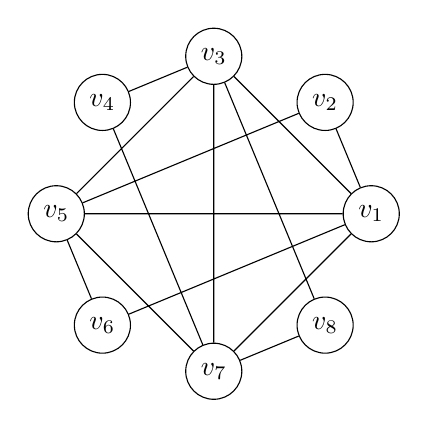
\begin{tikzpicture}[scale=2, bend angle=22.5]
\tikzstyle{every node}=[draw,shape=circle];
\foreach \i in {1,...,8}
{
\path (45*\i-45:1cm) node (v\i) {$v_\i$};
}
\draw
(v1) -- (v2) (v3) -- (v4) (v5) -- (v6) (v7) -- (v8)
(v1) -- (v3) (v3) -- (v5) (v5) -- (v7) (v7) -- (v1)
(v2) -- (v5) (v4) -- (v7) (v6) -- (v1) (v8) -- (v3)
(v1) -- (v5) (v3) -- (v7);
\end{tikzpicture}
\end{frame}

\begin{frame}[fragile]
	\begin{multicols}{2}
\inputminted[xleftmargin=1.5em]{latex}{tikz/binary_tree.tex}
	\end{multicols}
\end{frame}

\begin{frame}
	\centering
	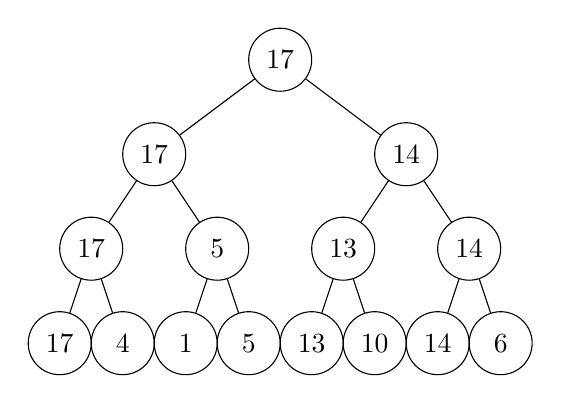
\begin{tikzpicture}[scale=0.8]
\tikzstyle{every node}=[draw,shape=circle,minimum size=0.8cm];
\node {17}[sibling distance=4cm]
child { node {17}[sibling distance=2cm]
	child {
		node {17}[sibling distance=1cm]
		child { node {17} }
		child { node {4} }
	}
	child {
		node {5}[sibling distance=1cm]
		child { node {1} }
		child { node {5} }
	}
}
child { node {14}[sibling distance=2cm]
	child {
		node {13}[sibling distance=1cm]
		child { node {13} }
		child { node {10} }
	}
	child {
		node {14}[sibling distance=1cm]
		child { node {14} }
		child { node {6} }
	}
};
\end{tikzpicture}
\end{frame}

\begin{frame}
The process of memorizing the code in TikZ is quite hard, so while you need to plot some graph with TikZ, it is highly recommended that you refer to the \myhref{http://www.texample.net/tikz/} for the codes of examples shown in it.
\end{frame}

\end{document}
